\clearpage
\section{البوابة العامة}
\label{sec:settings-feature-public-portal}

البوابة العامة هي الموقع الذي يدخله المتعاملون ليبحثوا عن خدمات المؤسسة ويقدموا طلباتهم ويتابعوها. والمتعامل هو أي شخص من خارج المؤسسة يستخدم هذه البوابة. تضبط هنا هوية البوابة وصفحتها الرئيسية وطرق التواصل ولغاتها، لذلك تعود إلى هذه الصفحة عند إطلاق البوابة وكلما تغيرت بيانات المؤسسة.

يفتح هذه الصفحة مالك المؤسسة ومن يحمل دور المسؤول. أما تبويب «المساحات» فله صلاحية خاصة تُمنح من الأدوار، فقد يصل إليه عضو لا يرى بقية التبويبات. وتبقى تعديلاتك مسودة تظهر في المعاينة فقط، ولا تصل إلى المتعاملين قبل الضغط على «نشر التغييرات».

\begin{rcnote}[مثال: شركة الأفق]
يكتب مسؤول النظام في شركة الأفق عنواناً واضحاً للبوابة، ثم يرتب عند ② قسم الخدمات قبل الإعلانات. يراجع النتيجة في المعاينة، ثم يضغط ④ لنشرها.
\end{rcnote}
\begin{figure}[H]
\centering
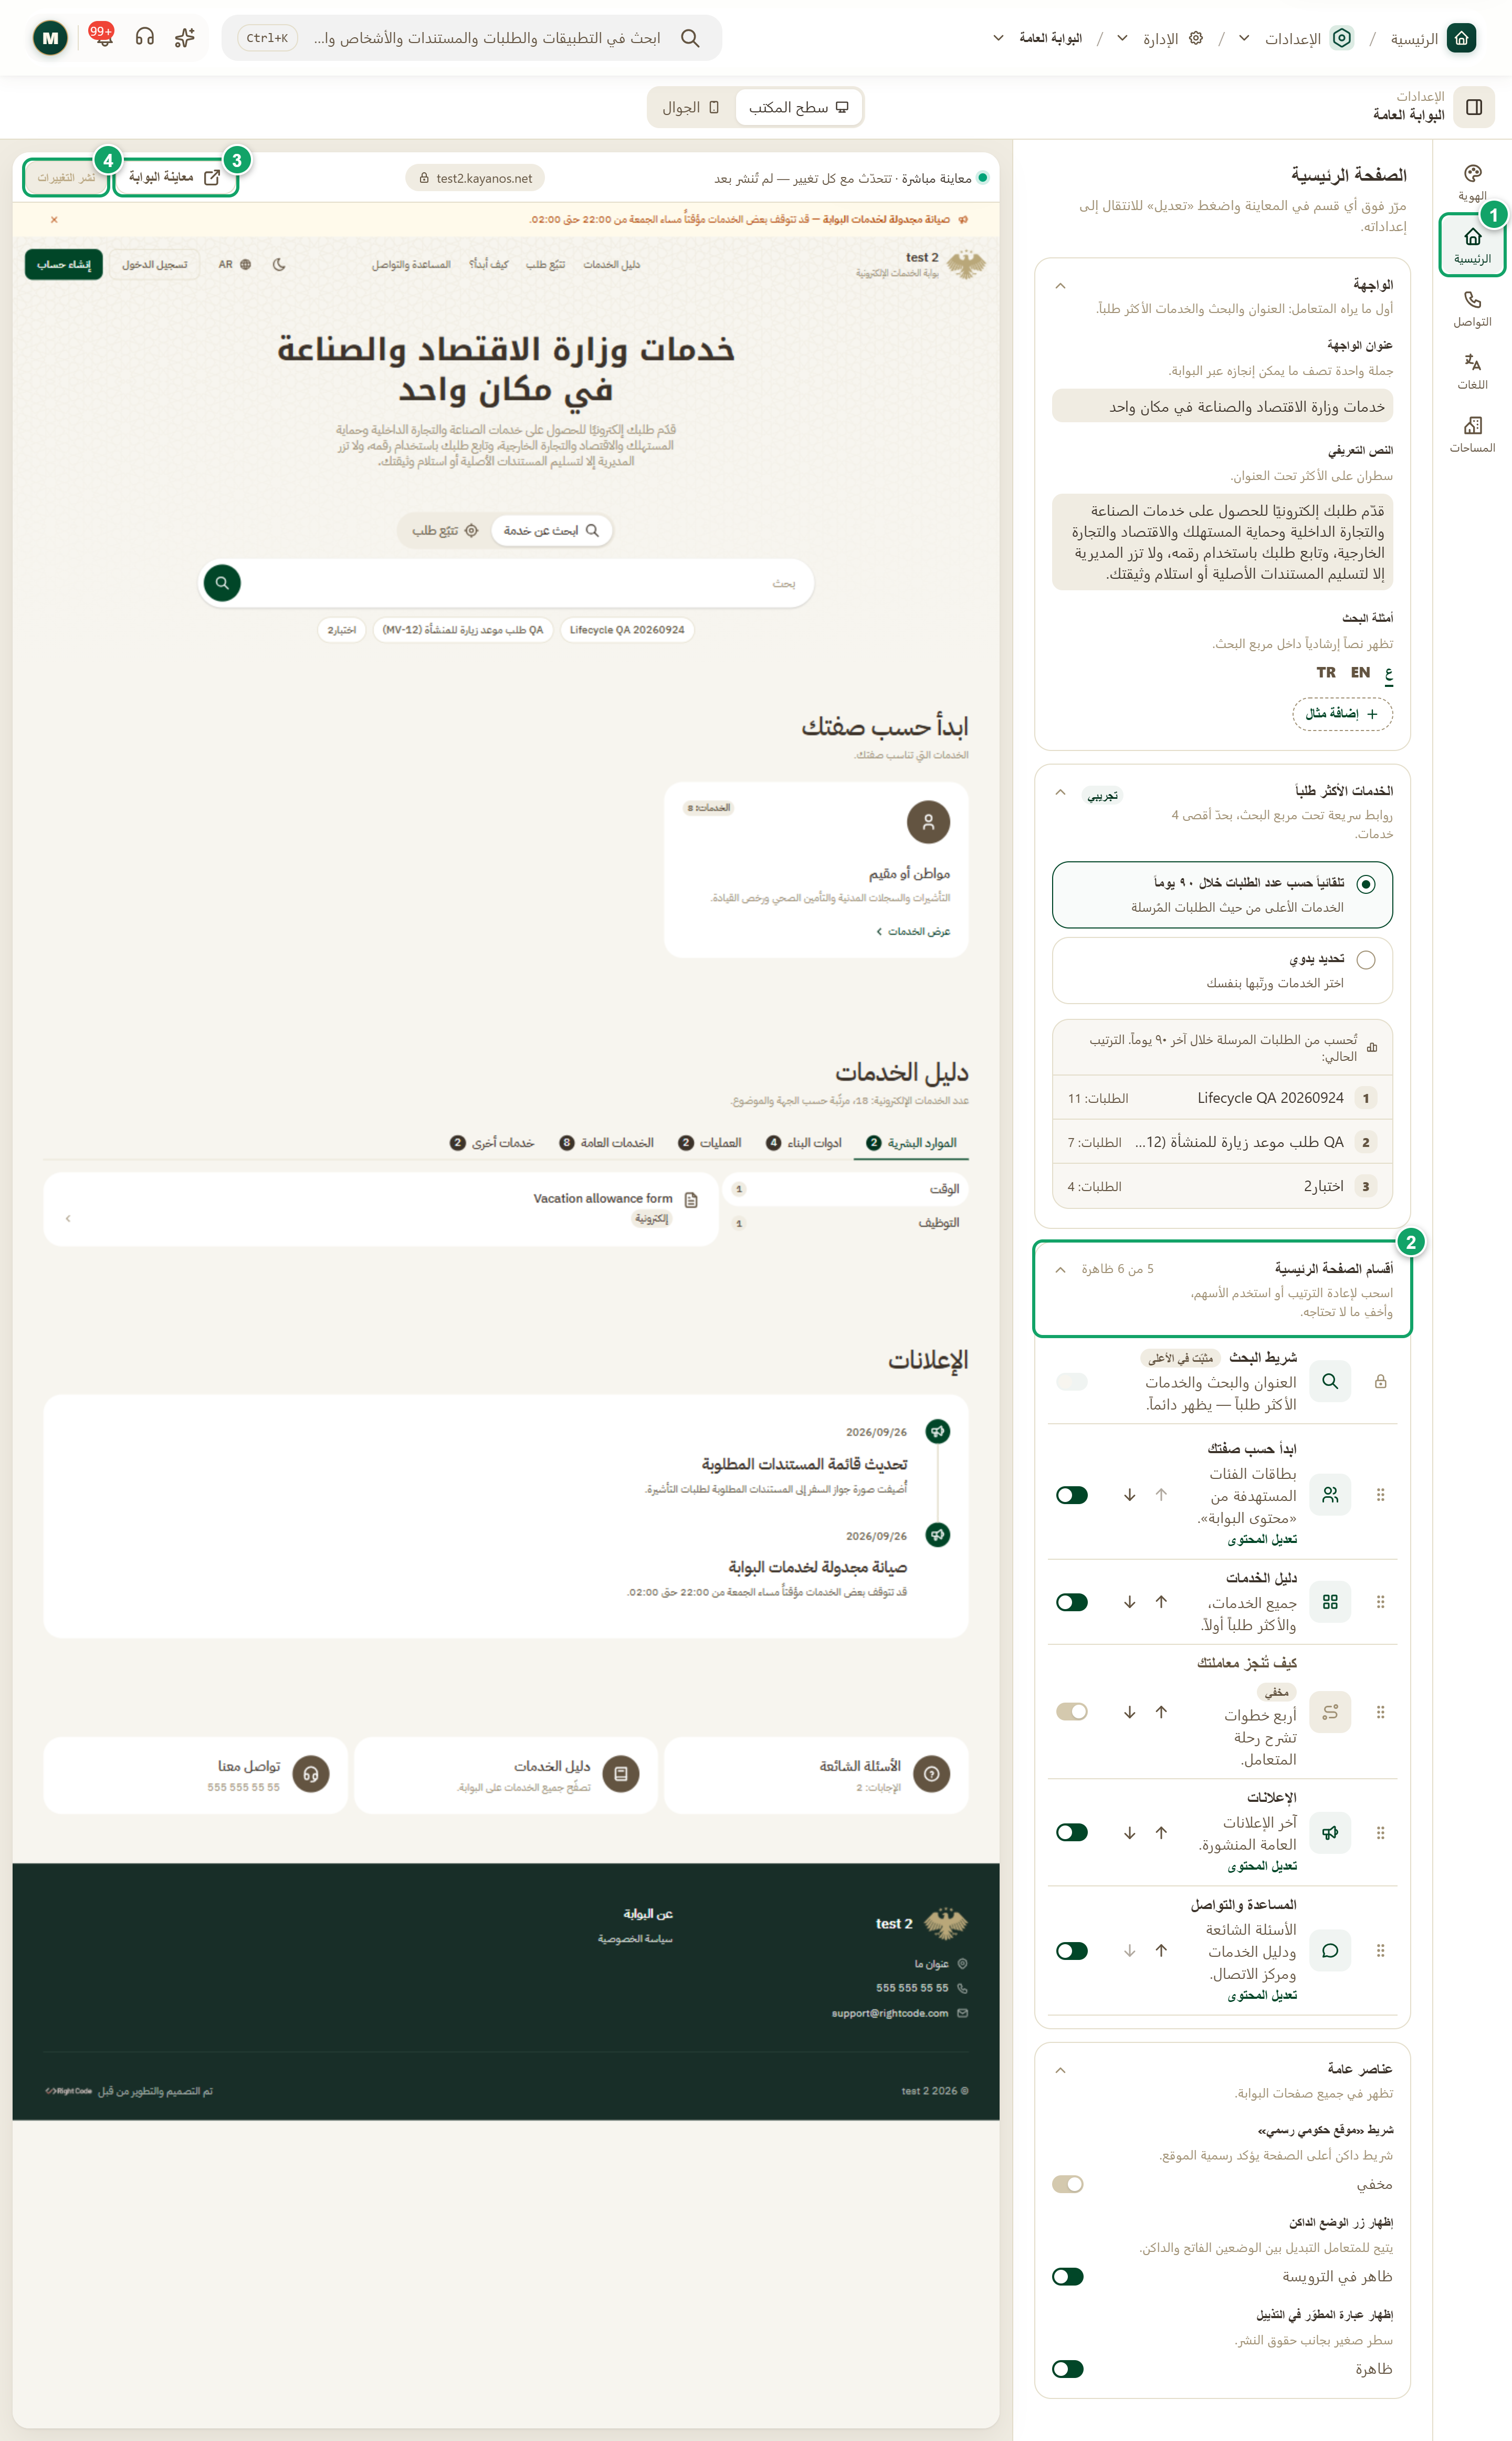
\includegraphics[width=0.95\linewidth,height=0.72\textheight,keepaspectratio]{figures/screens/ch08-public-portal-home-ar.png}
\caption{تبويب الرئيسية والمعاينة المباشرة}
\label{fig:settings-public-portal-home}
\shotnote{تعرض الصورة لوحة الإعدادات بجوار معاينة حية للبوابة، فترى أثر كل تغيير قبل نشره. المحتوى الظاهر بيانات اختبار. ① «الرئيسية». ② «أقسام الصفحة الرئيسية»: لتغيير ترتيب الأقسام وإخفاء ما لا تحتاج إليه؛ ويبقى شريط البحث ثابتاً في الأعلى. ③ «معاينة البوابة»: تفتح البوابة في نافذة جديدة. ④ «نشر التغييرات»: يبقى معطلاً حتى تعدّل شيئاً.}
\end{figure}

\begin{figure}[H]
\centering
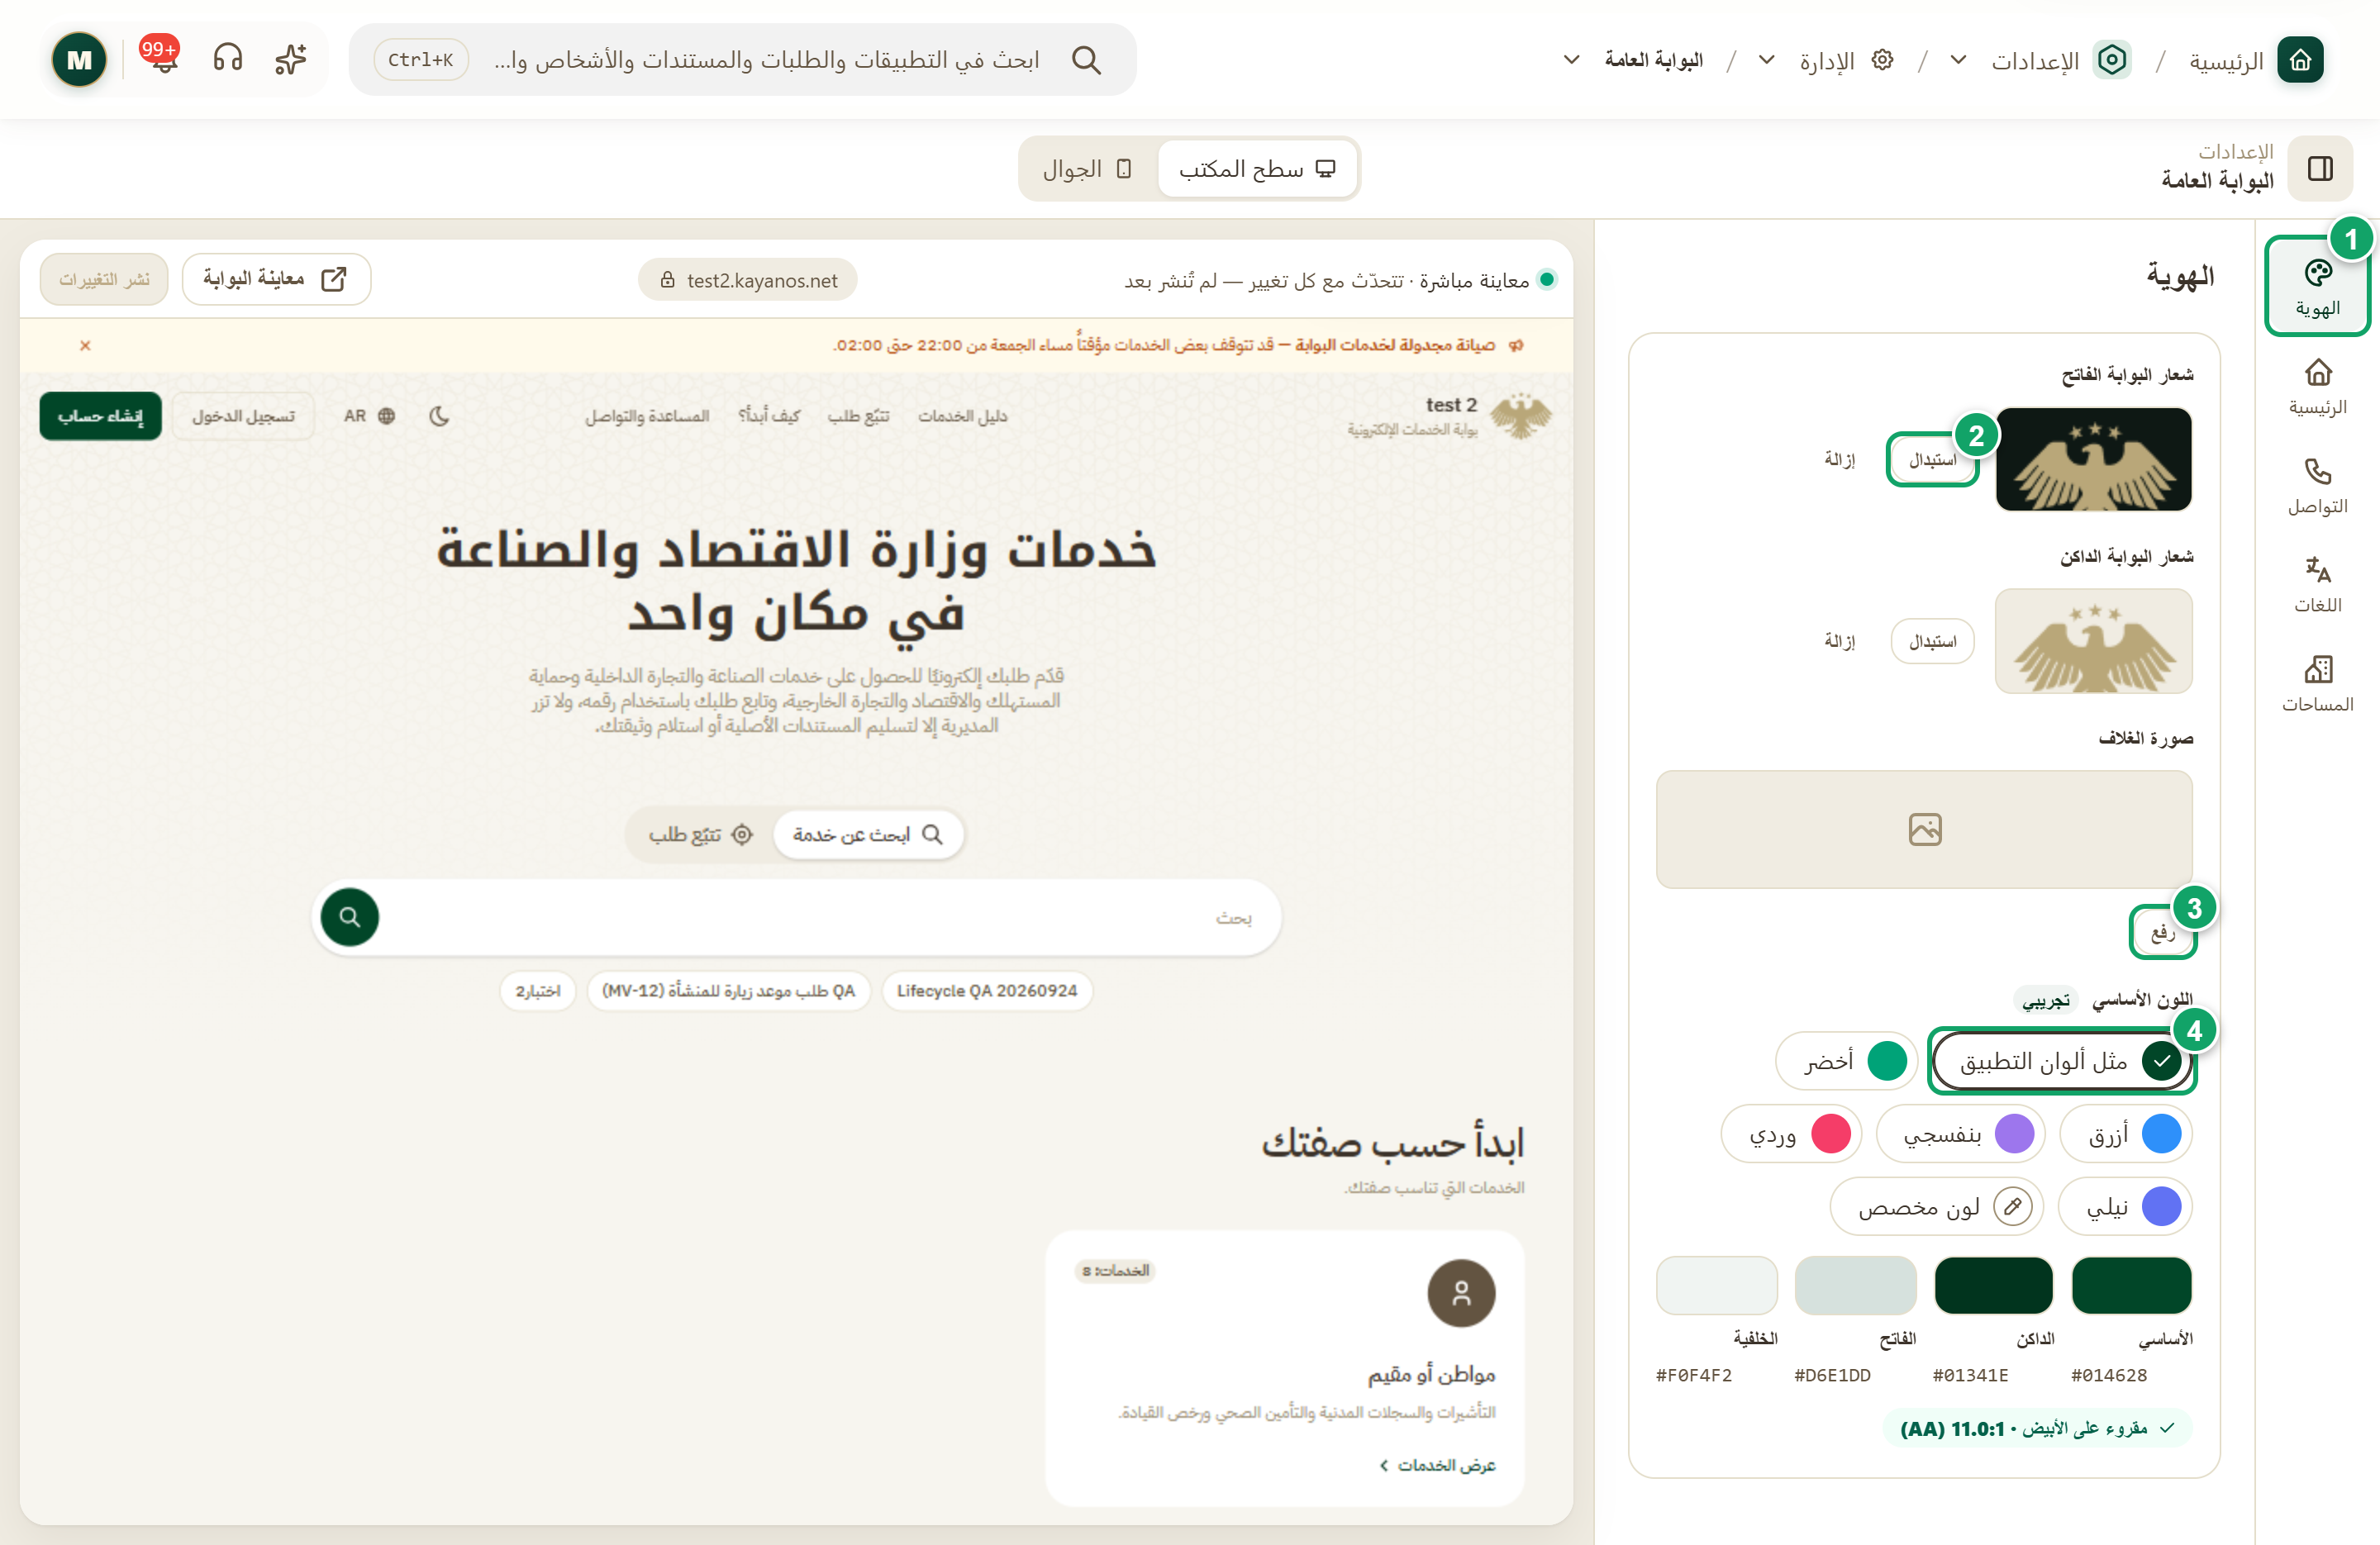
\includegraphics[width=0.95\linewidth,height=0.72\textheight,keepaspectratio]{figures/screens/ch08-public-portal-identity-ar.png}
\caption{تبويب الهوية}
\label{fig:settings-public-portal-identity}
\shotnote{يحدد هذا التبويب الصور واللون اللذين يميزان البوابة عن غيرها. تفحص الصفحة اللون المختار وتبين هل يبقى النص مقروءاً على الخلفية البيضاء. ① «الهوية». ② «استبدال»: لتغيير الشعار الفاتح الذي يظهر على الخلفيات الداكنة. ③ «رفع»: لإضافة صورة الغلاف. ④ «مثل ألوان التطبيق»: تجعل البوابة تتبع ألوان التطبيق، ويمكنك اختيار لون آخر بجواره.}
\end{figure}

\begin{figure}[H]
\centering
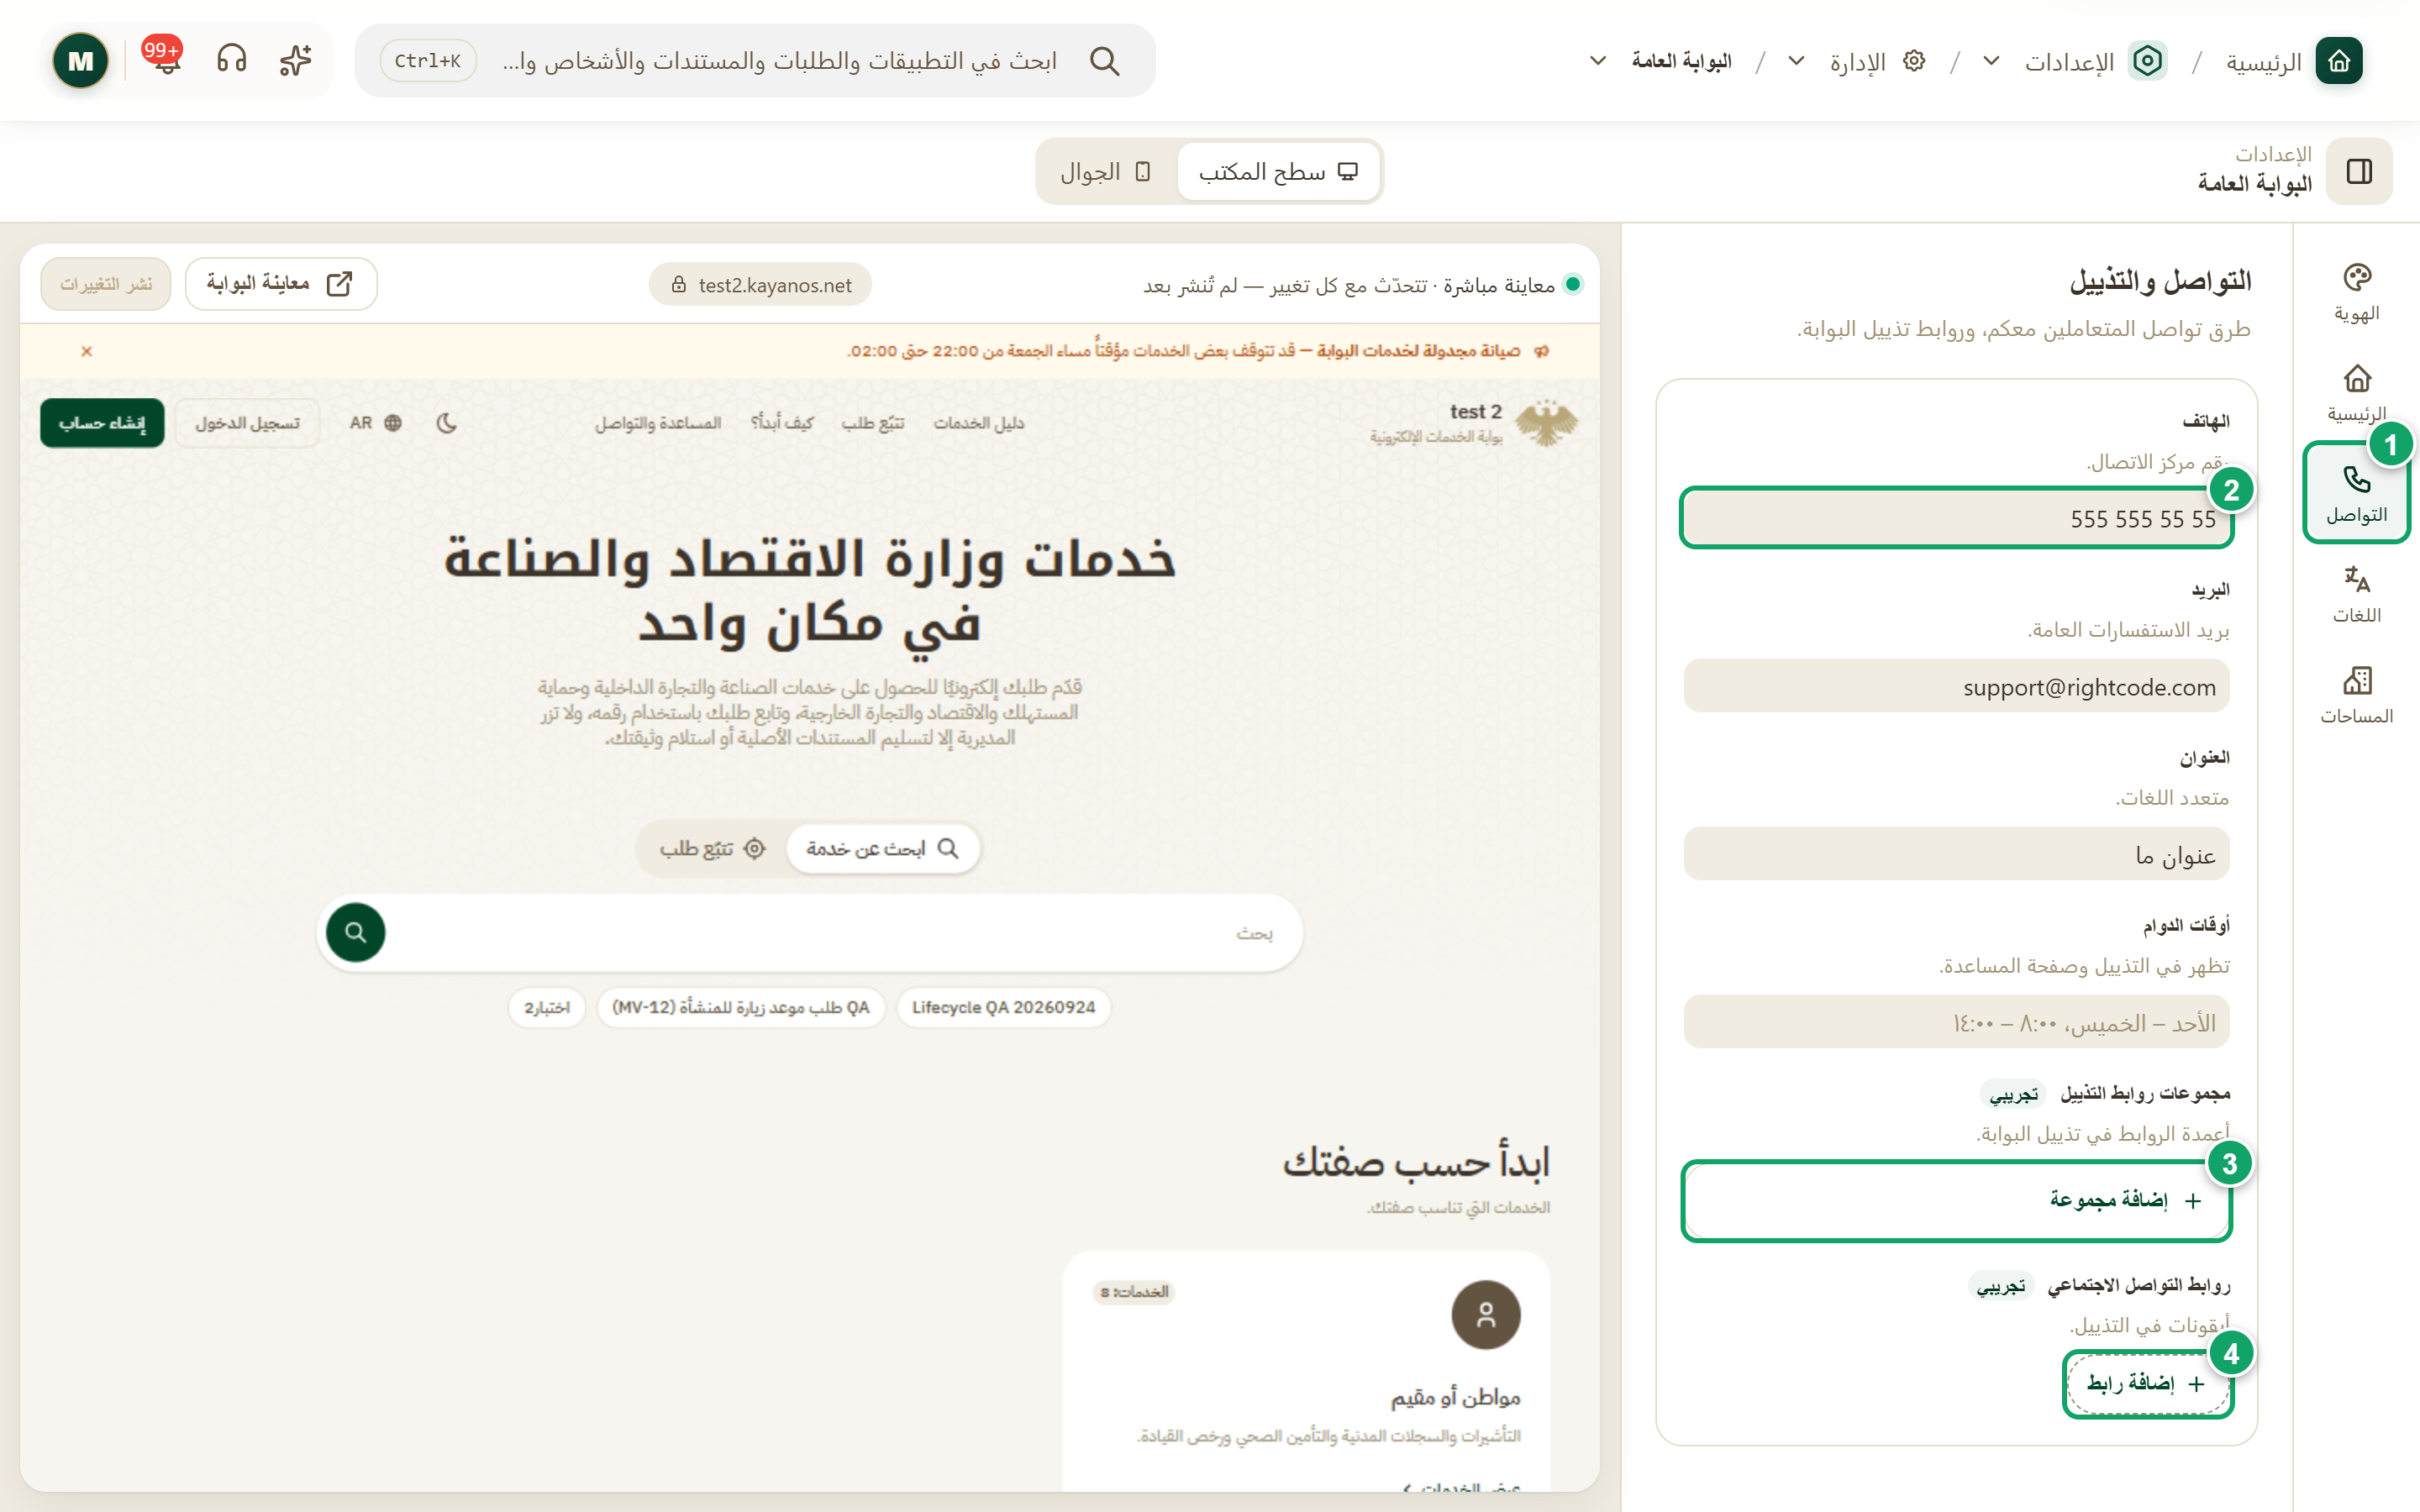
\includegraphics[width=0.95\linewidth,height=0.72\textheight,keepaspectratio]{figures/screens/ch08-public-portal-contact-ar.png}
\caption{تبويب التواصل}
\label{fig:settings-public-portal-contact}
\shotnote{يجمع هذا التبويب ما يحتاج إليه المتعامل للوصول إلى مؤسستك، ويظهر معظمه في تذييل البوابة، وهو الجزء الثابت أسفل كل صفحة. لا يقبل النشر رابطاً ناقصاً؛ فلكل رابط اسم وعنوان صحيح. ① «التواصل». ② حقل «الهاتف»: رقم مركز الاتصال. ③ «إضافة مجموعة»: لإضافة عمود روابط إلى التذييل. ④ «إضافة رابط»: لإضافة رابط إلى حساب في شبكات التواصل الاجتماعي.}
\end{figure}

\begin{figure}[H]
\centering
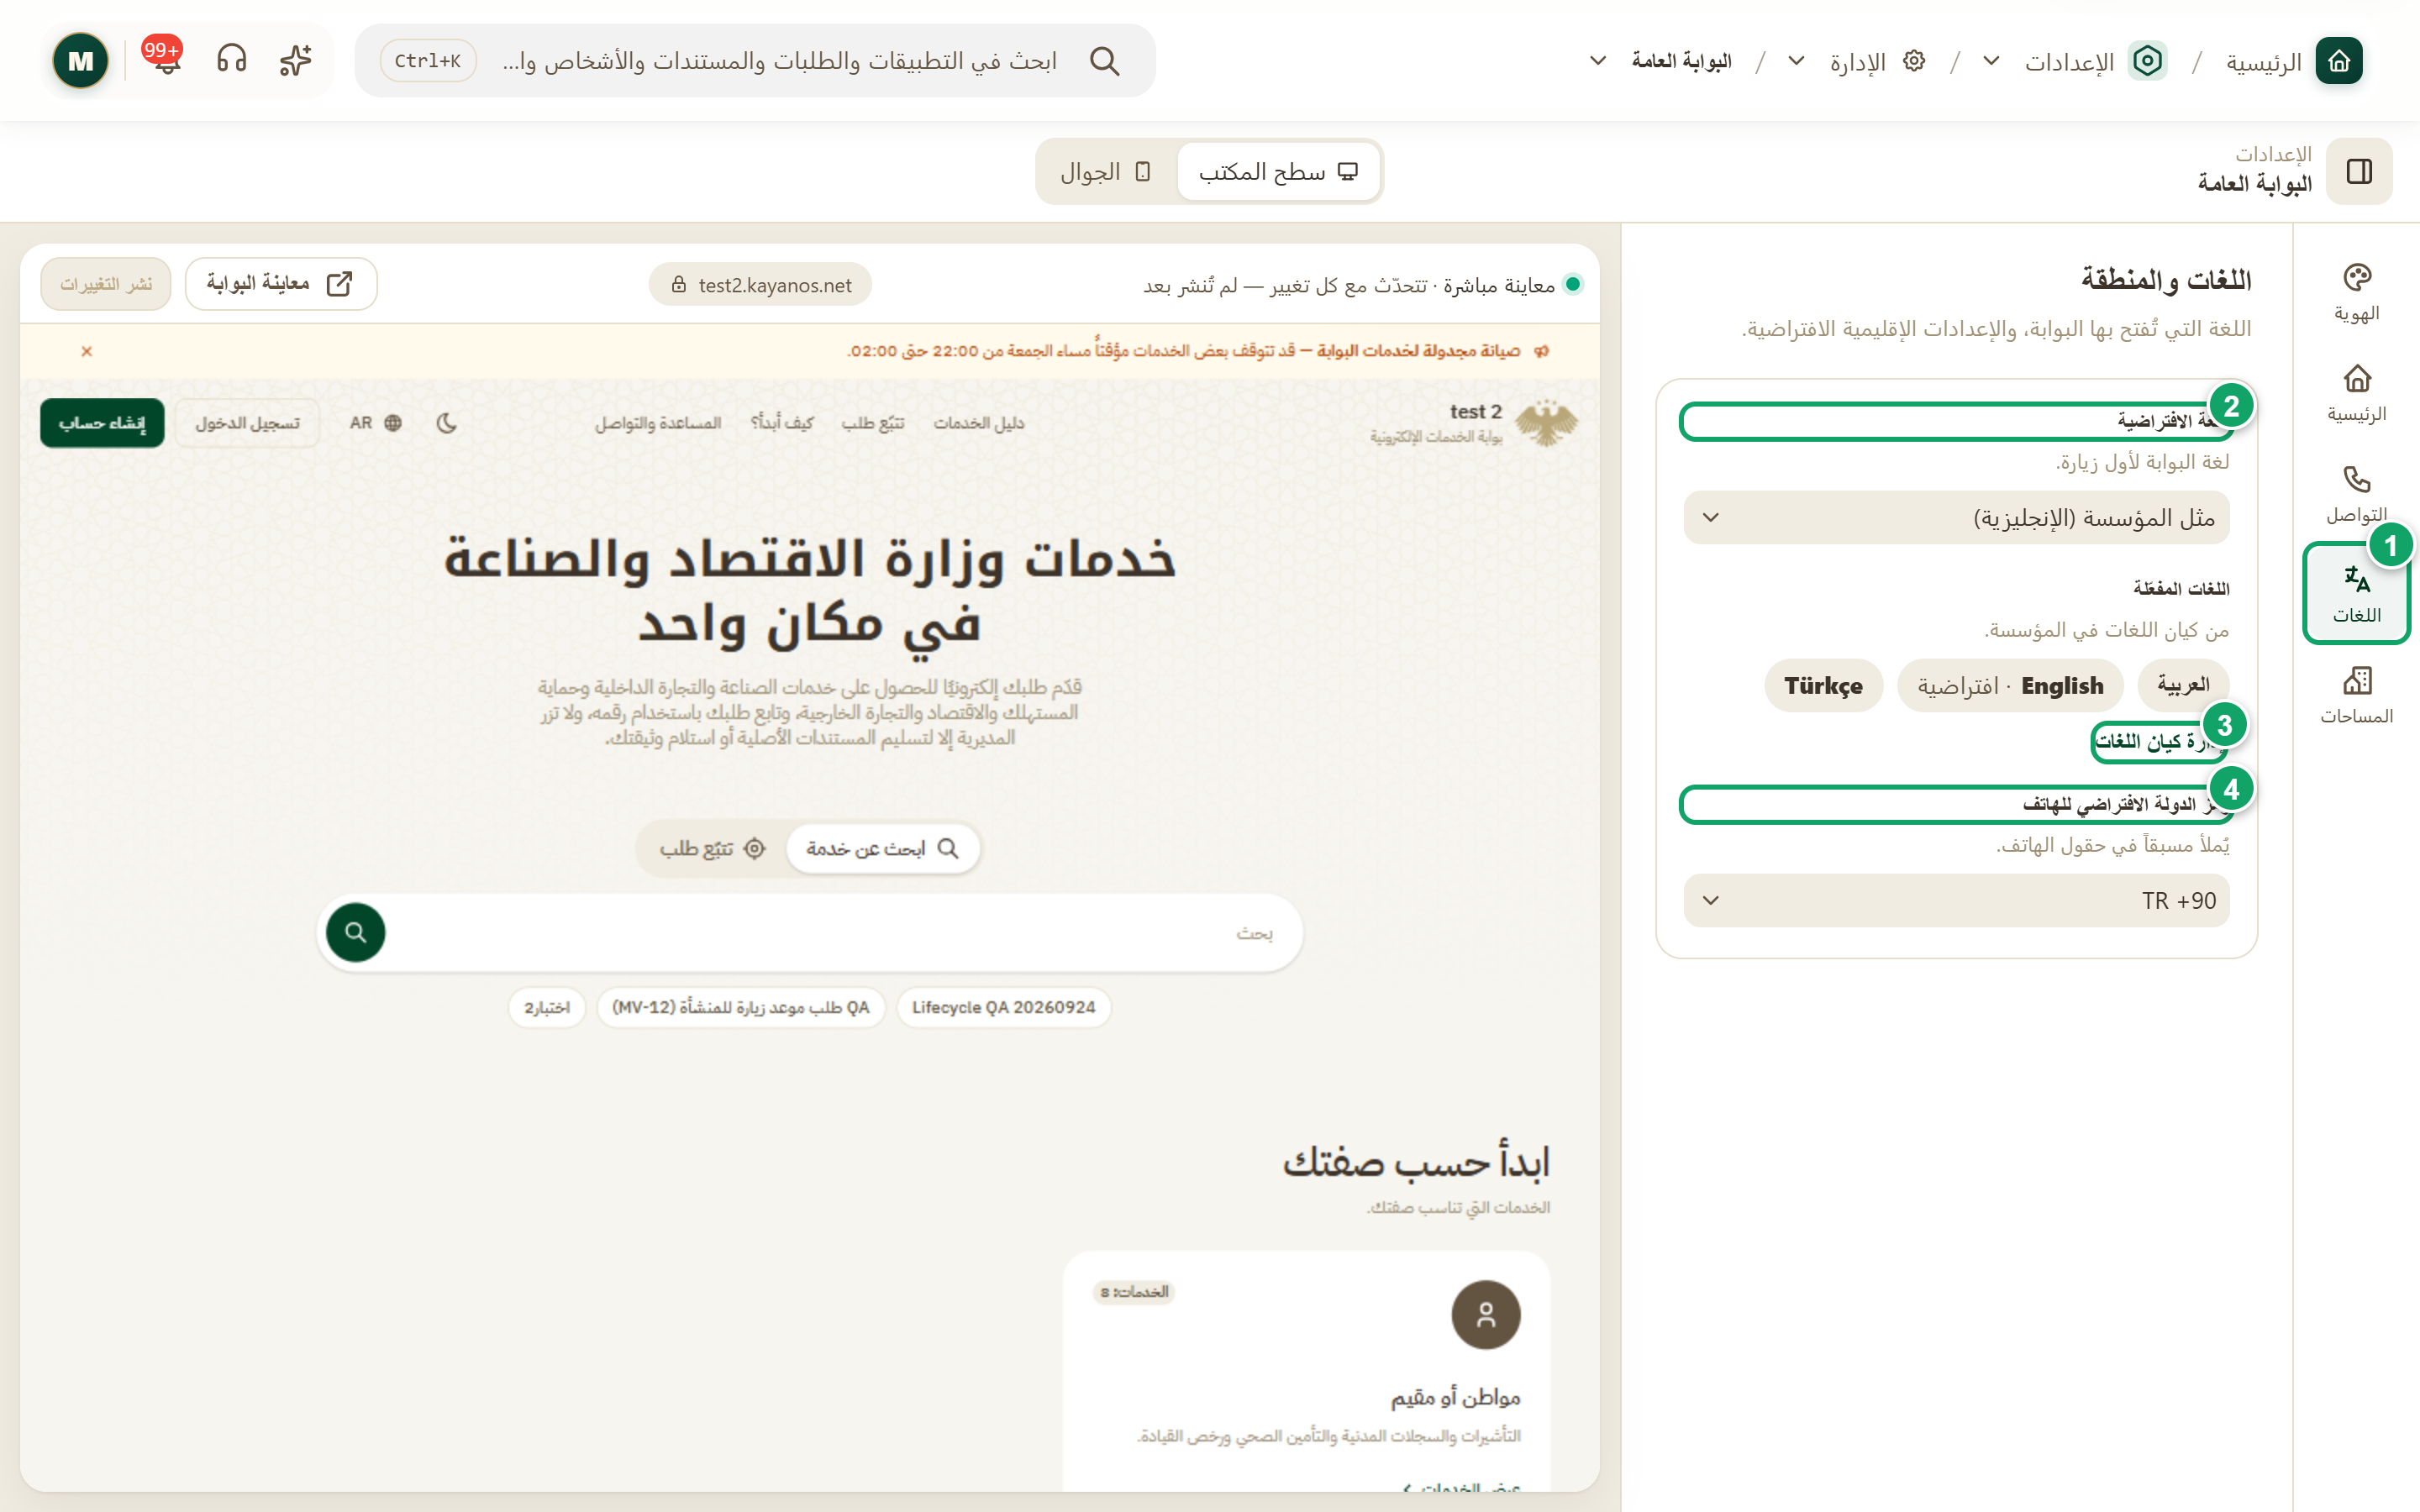
\includegraphics[width=0.95\linewidth,height=0.72\textheight,keepaspectratio]{figures/screens/ch08-public-portal-languages-ar.png}
\caption{تبويب اللغات}
\label{fig:settings-public-portal-languages}
\shotnote{يحدد هذا التبويب اللغة التي يراها الزائر أول مرة، أما قائمة اللغات نفسها فتأتي من لغات المؤسسة ولا تُعدَّل هنا. ① «اللغات». ② «اللغة الافتراضية». ③ «إدارة كيان اللغات»: تنقلك إلى صفحة لغات المؤسسة. ④ «رمز الدولة الافتراضي للهاتف»: يُملأ مسبقاً في حقول الهاتف.}
\end{figure}

\begin{figure}[H]
\centering
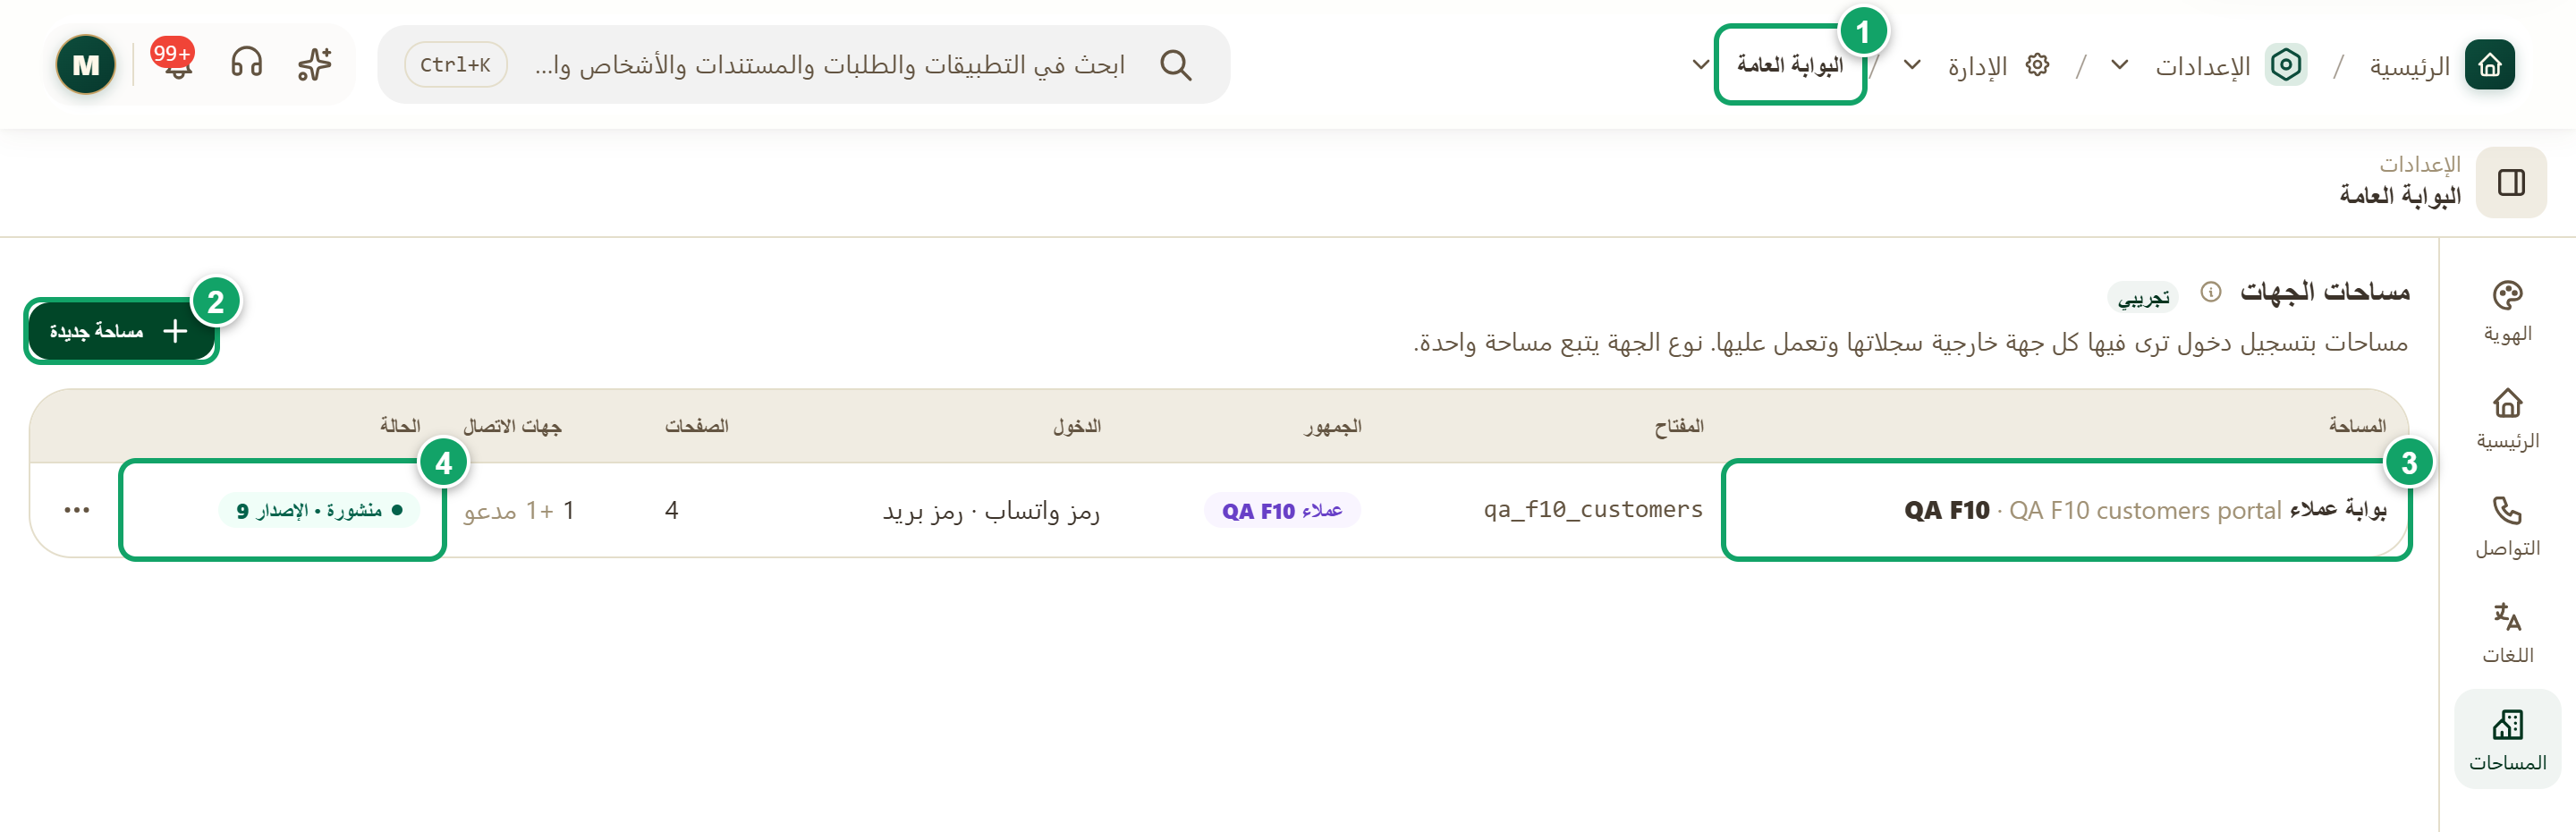
\includegraphics[width=0.95\linewidth,height=0.72\textheight,keepaspectratio]{figures/screens/ch08-public-portal-spaces-ar.png}
\caption{تبويب المساحات}
\label{fig:settings-public-portal-spaces}
\shotnote{المساحة منطقة يسجل فيها طرف خارجي، كعميل أو مورد، دخوله ليرى سجلاته ويعمل عليها. تُنشر كل مساحة وحدها، فلا يشملها زر «نشر التغييرات». الصف الظاهر مساحة اختبار. ① «المساحات». ② «مساحة جديدة». ③ اسم المساحة. ④ حالة المساحة ورقم إصدارها المنشور.}
\end{figure}

\begin{table}[H]
\centering
\caption{ماذا تسجل في البوابة العامة؟}
\label{tab:settings-public-portal-fields}
\begin{tabularx}{\linewidth}{R{4.2cm} Y}
\rcHeaderRow
\thh{التبويب} & \thh{ما الذي تضبطه؟}\\
«الهوية» & «شعار البوابة الفاتح» و«شعار البوابة الداكن» و«صورة الغلاف» بحجم لا يتجاوز 5 ميغابايت لكل صورة، ثم «اللون الأساسي».\\
«الرئيسية» & «الواجهة»: «عنوان الواجهة» و«النص التعريفي» و«أمثلة البحث». «الخدمات الأكثر طلباً»: تلقائياً بحسب طلبات آخر 90 يوماً أو «تحديد يدوي»، وبحد أقصى أربع خدمات. «أقسام الصفحة الرئيسية». «عناصر عامة»: شريط «موقع حكومي رسمي» وزر الوضع الداكن وعبارة المطوّر في التذييل.\\
«التواصل» & «الهاتف» و«البريد» و«العنوان» و«أوقات الدوام»، ثم «مجموعات روابط التذييل» بحد أقصى أربع مجموعات وثمانية روابط لكل مجموعة، و«روابط التواصل الاجتماعي» بحد أقصى ثمانية روابط.\\
«اللغات» & «اللغة الافتراضية»، وتتبع لغة المؤسسة ما لم تختر غيرها، و«رمز الدولة الافتراضي للهاتف». وتظهر «اللغات المفعّلة» للاطلاع.\\
«المساحات» & قائمة «مساحات الجهات»، ومنها تُنشأ المساحة وتُعدَّل أقسامها: «الجمهور»، و«تسجيل الدخول»، و«جهات الاتصال والأدوار»، و«الصفحات»، و«أنواع السجلات»، و«الإجراءات»، و«المصادقات»، و«الإشعارات»، و«الهوية»، و«الأمان».\\
\end{tabularx}
\end{table}

\begin{enumerate}
\item افتح «الإعدادات»، ثم «البوابة العامة».
\item اختر التبويب الذي تريد تعديله من العمود الجانبي، وعدّل قيمه.
\item راجع النتيجة في المعاينة، وبدّل بين «سطح المكتب» و«الجوال» لترى البوابة على الشاشتين.
\item مرّر فوق أي قسم في المعاينة واضغط «تعديل» إذا أردت الانتقال مباشرة إلى إعداداته.
\item اضغط «نشر التغييرات». يشمل النشر تعديلات التبويبات الأربعة الأولى معاً.
\end{enumerate}

\textbf{تحقق:} تظهر عبارة «تم الحفظ» بجوار زر النشر. اضغط «معاينة البوابة» وتأكد أن تعديلك ظاهر في البوابة. وإذا نقلتك الصفحة إلى تبويب «التواصل» مع رسالة خطأ، فأكمل رابط التذييل الناقص أو احذفه ثم انشر مجدداً.

\clearpage
\section{محتوى البوابة}
\label{sec:settings-feature-portal-content}

بينما تضبط صفحة «البوابة العامة» الشكل العام، تحمل هذه الصفحة ما يقرؤه المتعامل: بطاقات الفئات المستهدفة، والصفحات الطويلة كسياسة الخصوصية، والأسئلة الشائعة، والإعلانات. والفئة المستهدفة مجموعة من الخدمات تجمعها صفة المتعامل، مثل المستثمر أو مركز التدريب.

استخدم هذه الصفحة كلما أردت إضافة نص أو تحديثه دون تغيير إعدادات البوابة. يفتحها مالك المؤسسة ومن يحمل دور المسؤول. ولا تحتاج عناصرها إلى زر النشر: يُحفظ كل عنصر وحده، ويؤثر مفتاح الإظهار في الجدول فور الضغط عليه.

\begin{rcnote}[مثال: شركة الأفق]
يضيف مسؤول النظام إعلاناً عن إغلاق فرع حلب ليوم واحد، ويختار عند ② إظهاره شريطاً في كل الصفحات. يحدد موعديه عند ③، ثم يتأكد من تشغيل المفتاح عند ④ قبل الحفظ.
\end{rcnote}
\begin{figure}[H]
\centering
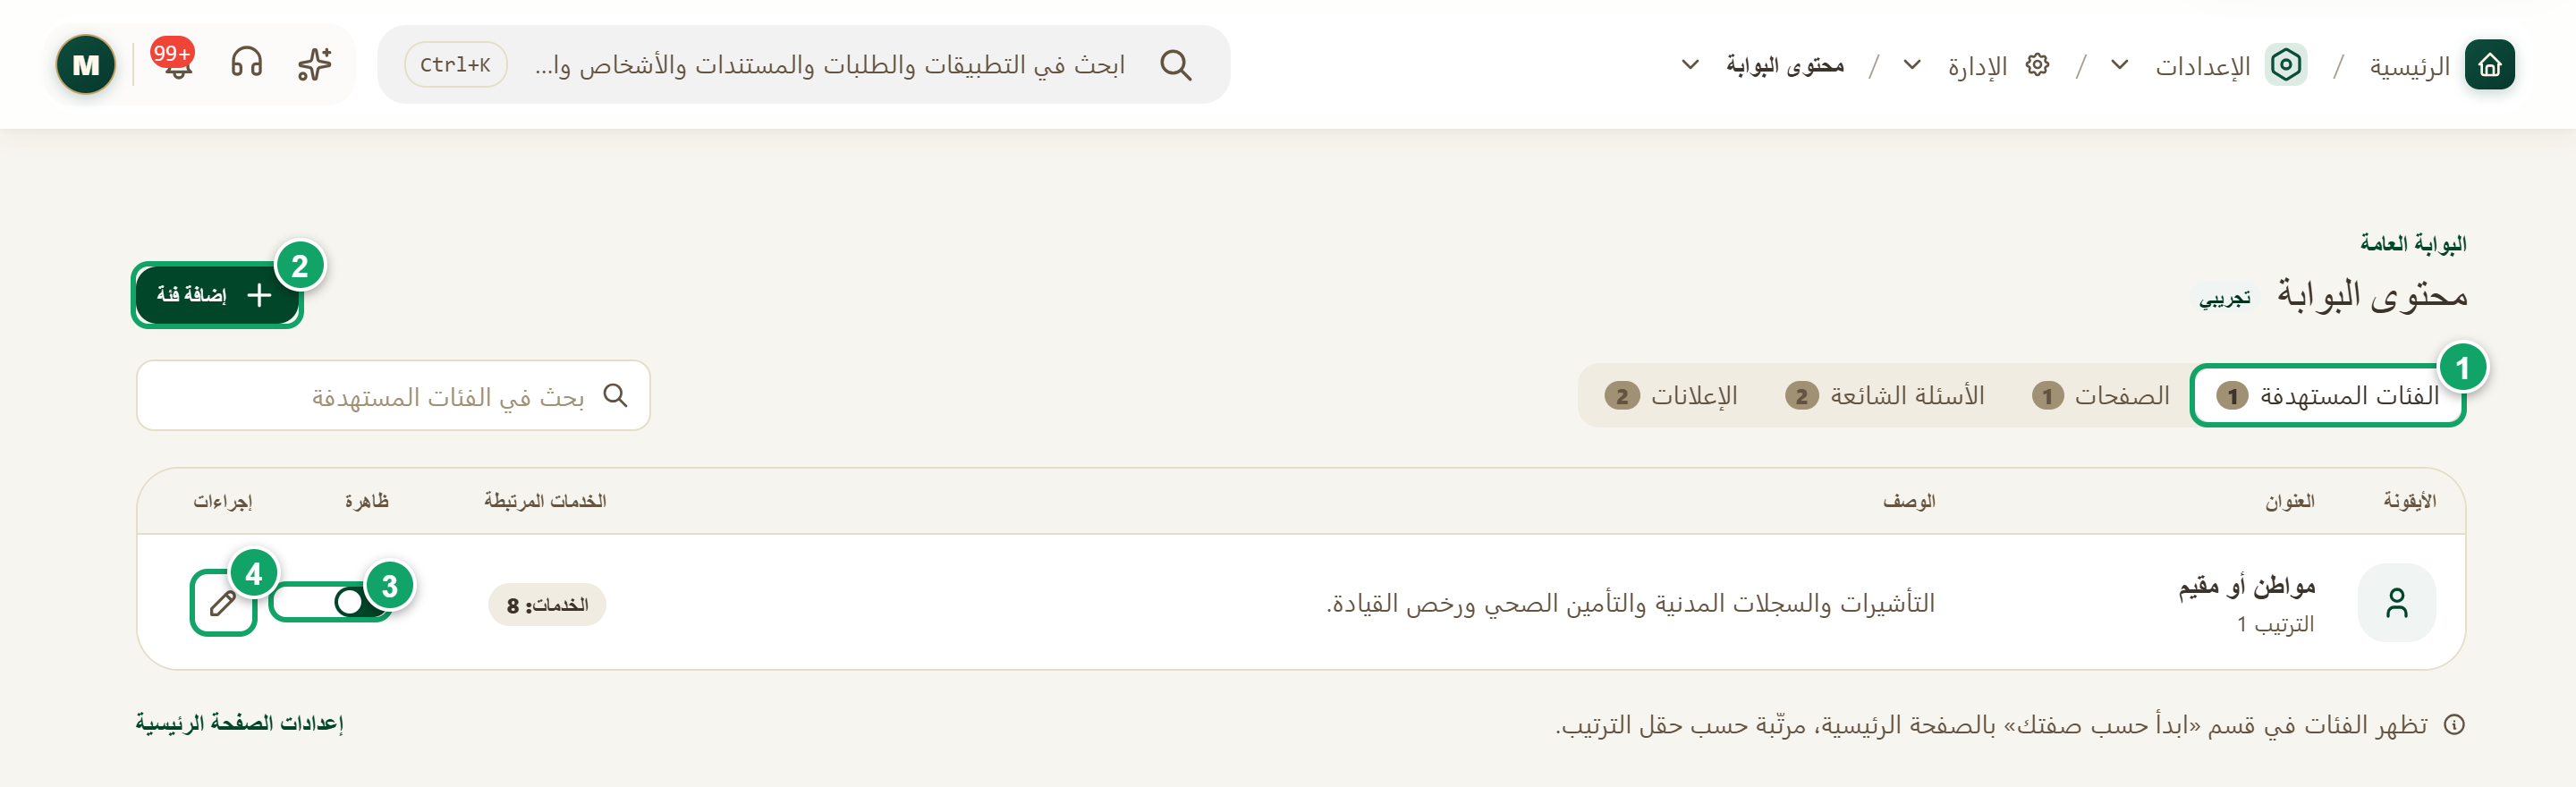
\includegraphics[width=0.95\linewidth,height=0.72\textheight,keepaspectratio]{figures/screens/ch08-portal-content-audience-ar.png}
\caption{الفئات المستهدفة}
\label{fig:settings-portal-content-audience}
\shotnote{تظهر الفئات في صورة بطاقات في قسم «ابدأ حسب صفتك» بالصفحة الرئيسية، فيصل المتعامل إلى خدماته دون أن يعرف أسماءها. الصف الظاهر بيانات اختبار. ① «الفئات المستهدفة». ② «إضافة فئة». ③ مفتاح «ظاهرة»: يخفي البطاقة أو يظهرها فوراً. ④ زر التعديل.}
\end{figure}

\begin{figure}[H]
\centering
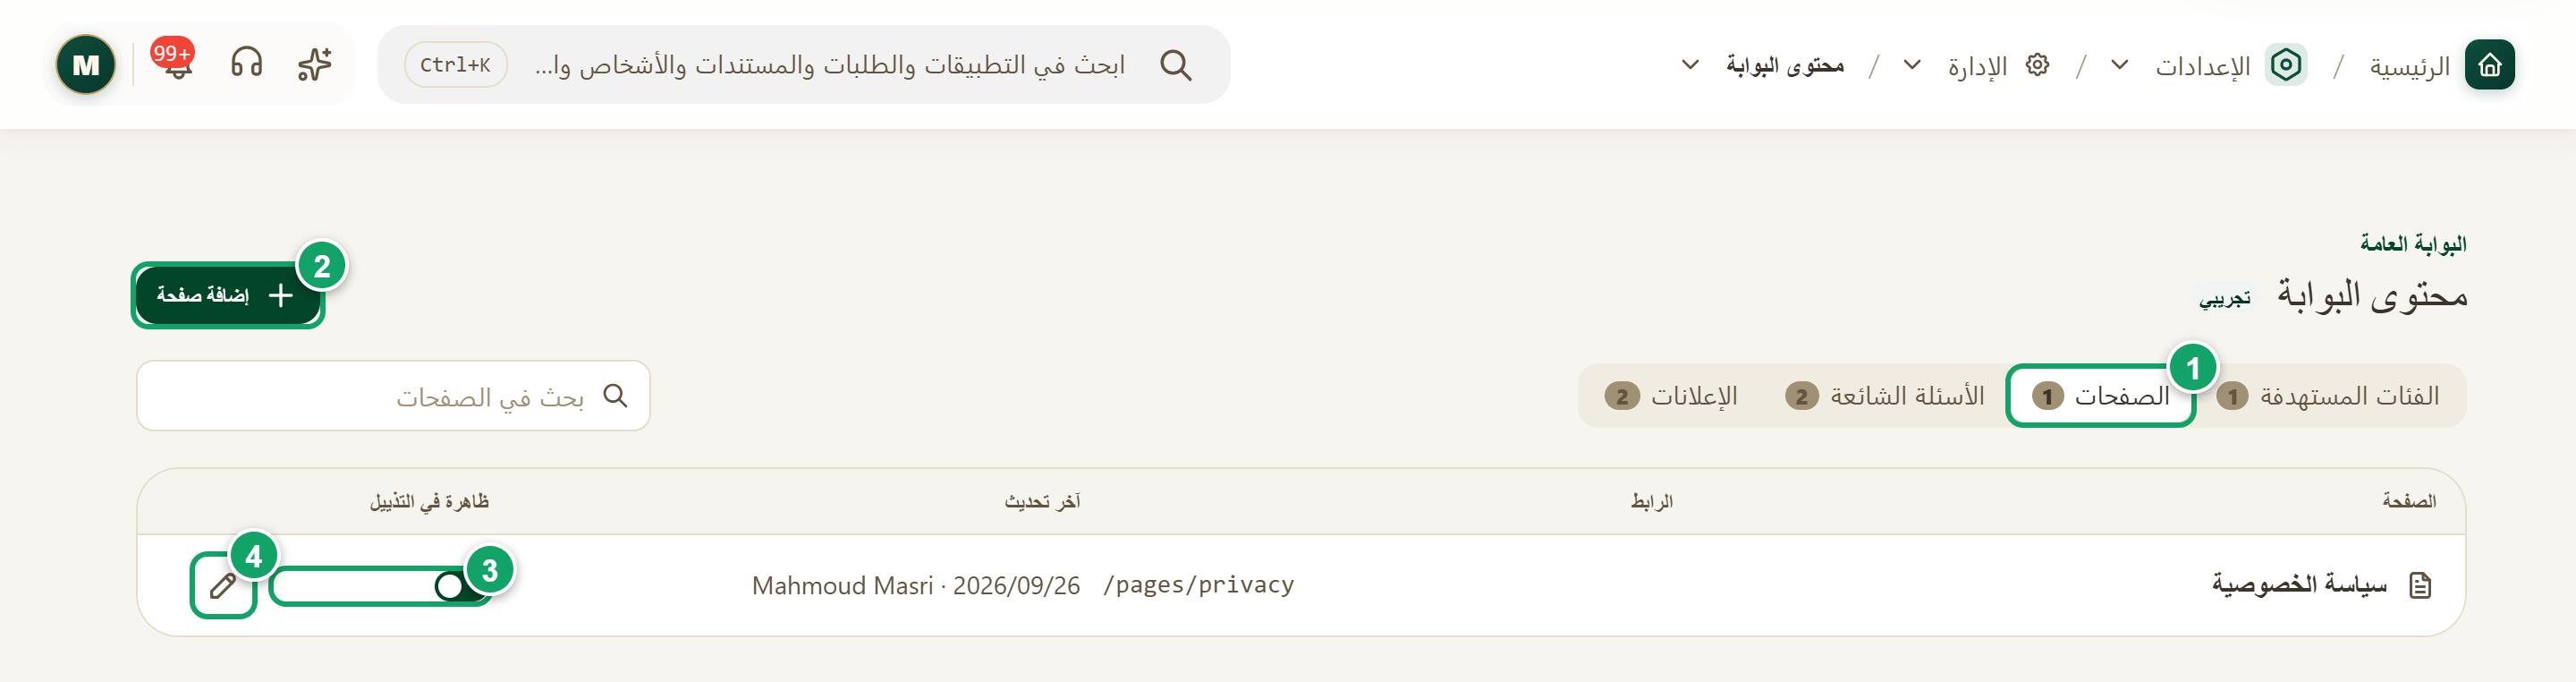
\includegraphics[width=0.95\linewidth,height=0.72\textheight,keepaspectratio]{figures/screens/ch08-portal-content-page-ar.png}
\caption{الصفحات}
\label{fig:settings-portal-content-page}
\shotnote{تحمل الصفحات النصوص الطويلة، ولكل صفحة رابط ثابت يعرضه الجدول. يتحكم المفتاح في ظهورها ضمن التذييل فقط، فتبقى متاحة لمن يملك رابطها. ① «الصفحات». ② «إضافة صفحة». ③ مفتاح «ظاهرة في التذييل». ④ زر التعديل.}
\end{figure}

\begin{figure}[H]
\centering
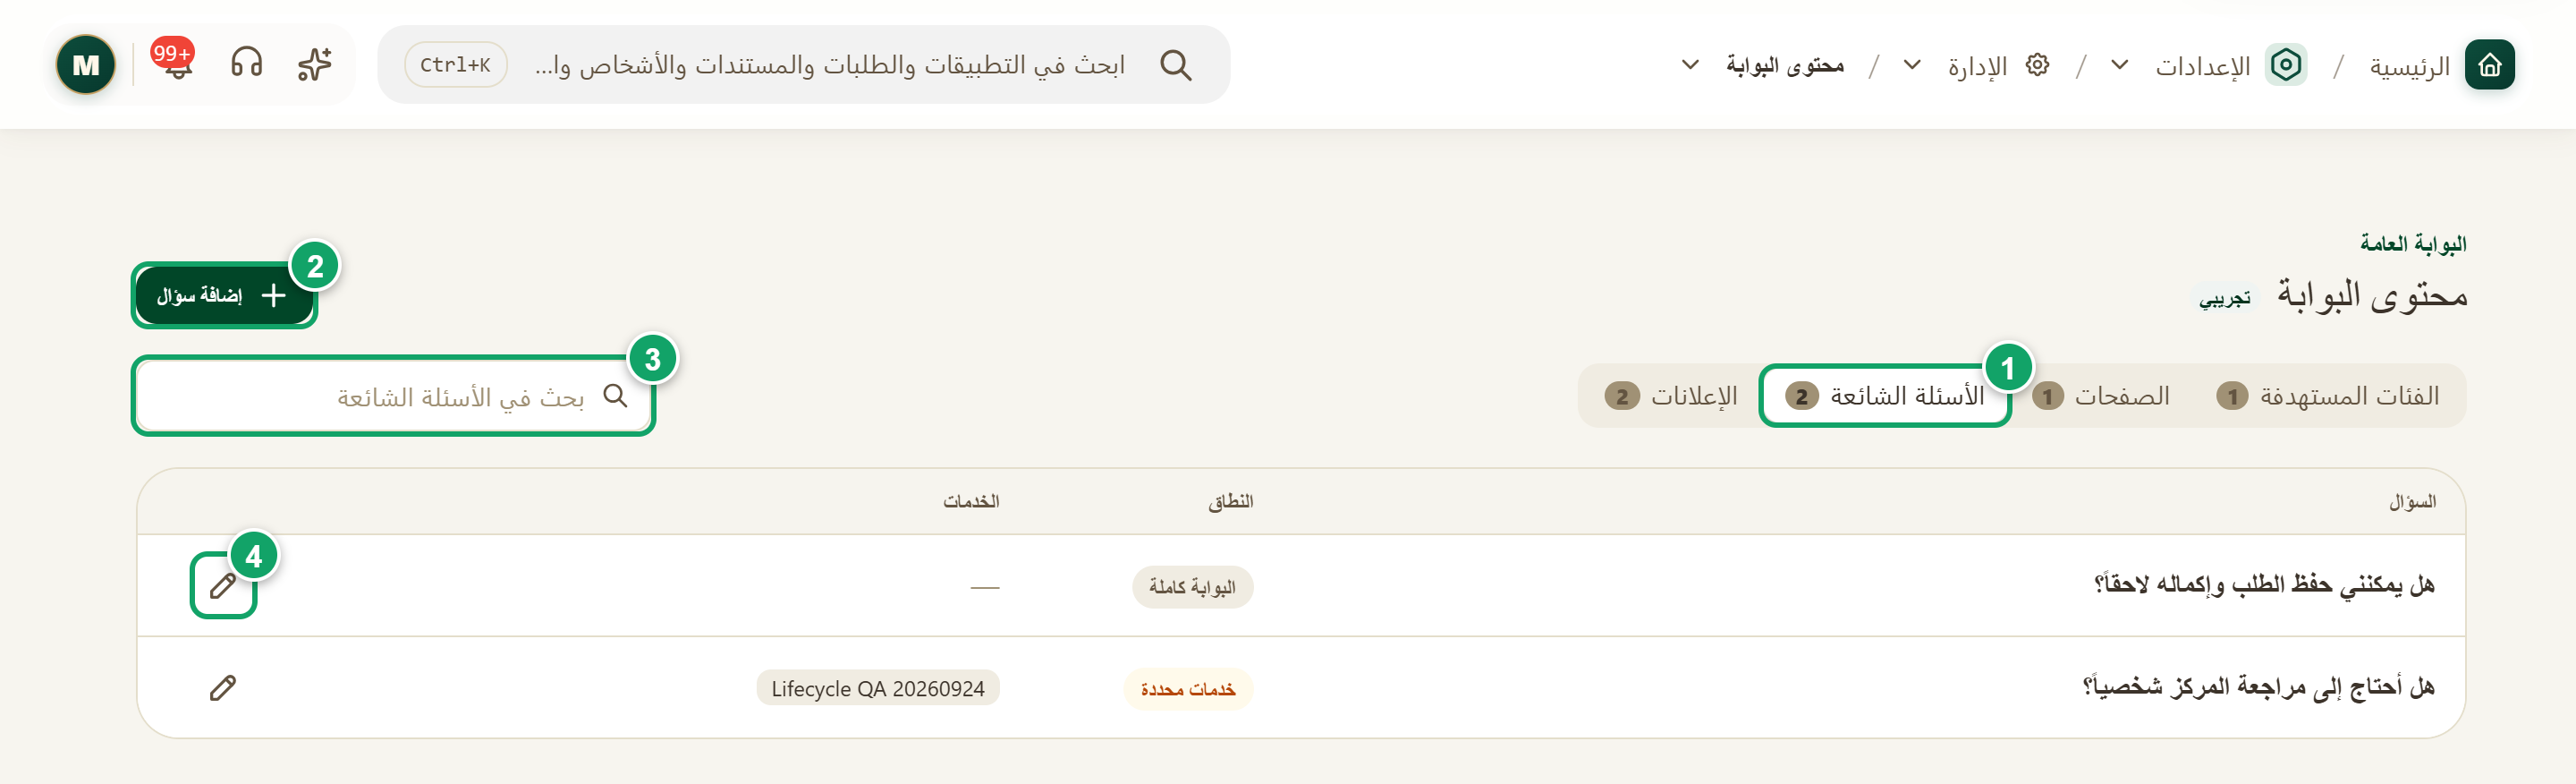
\includegraphics[width=0.95\linewidth,height=0.72\textheight,keepaspectratio]{figures/screens/ch08-portal-content-faq-ar.png}
\caption{الأسئلة الشائعة}
\label{fig:settings-portal-content-faq}
\shotnote{يحدد «النطاق» أين يظهر السؤال: في صفحة المساعدة وحدها، أو معها على خدمات تطبيق أو خدمات محددة. لذلك يصل السؤال المرتبط بخدمة إلى من يتقدم بطلبها فعلاً. ① «الأسئلة الشائعة». ② «إضافة سؤال». ③ حقل البحث. ④ زر التعديل.}
\end{figure}

\begin{figure}[H]
\centering
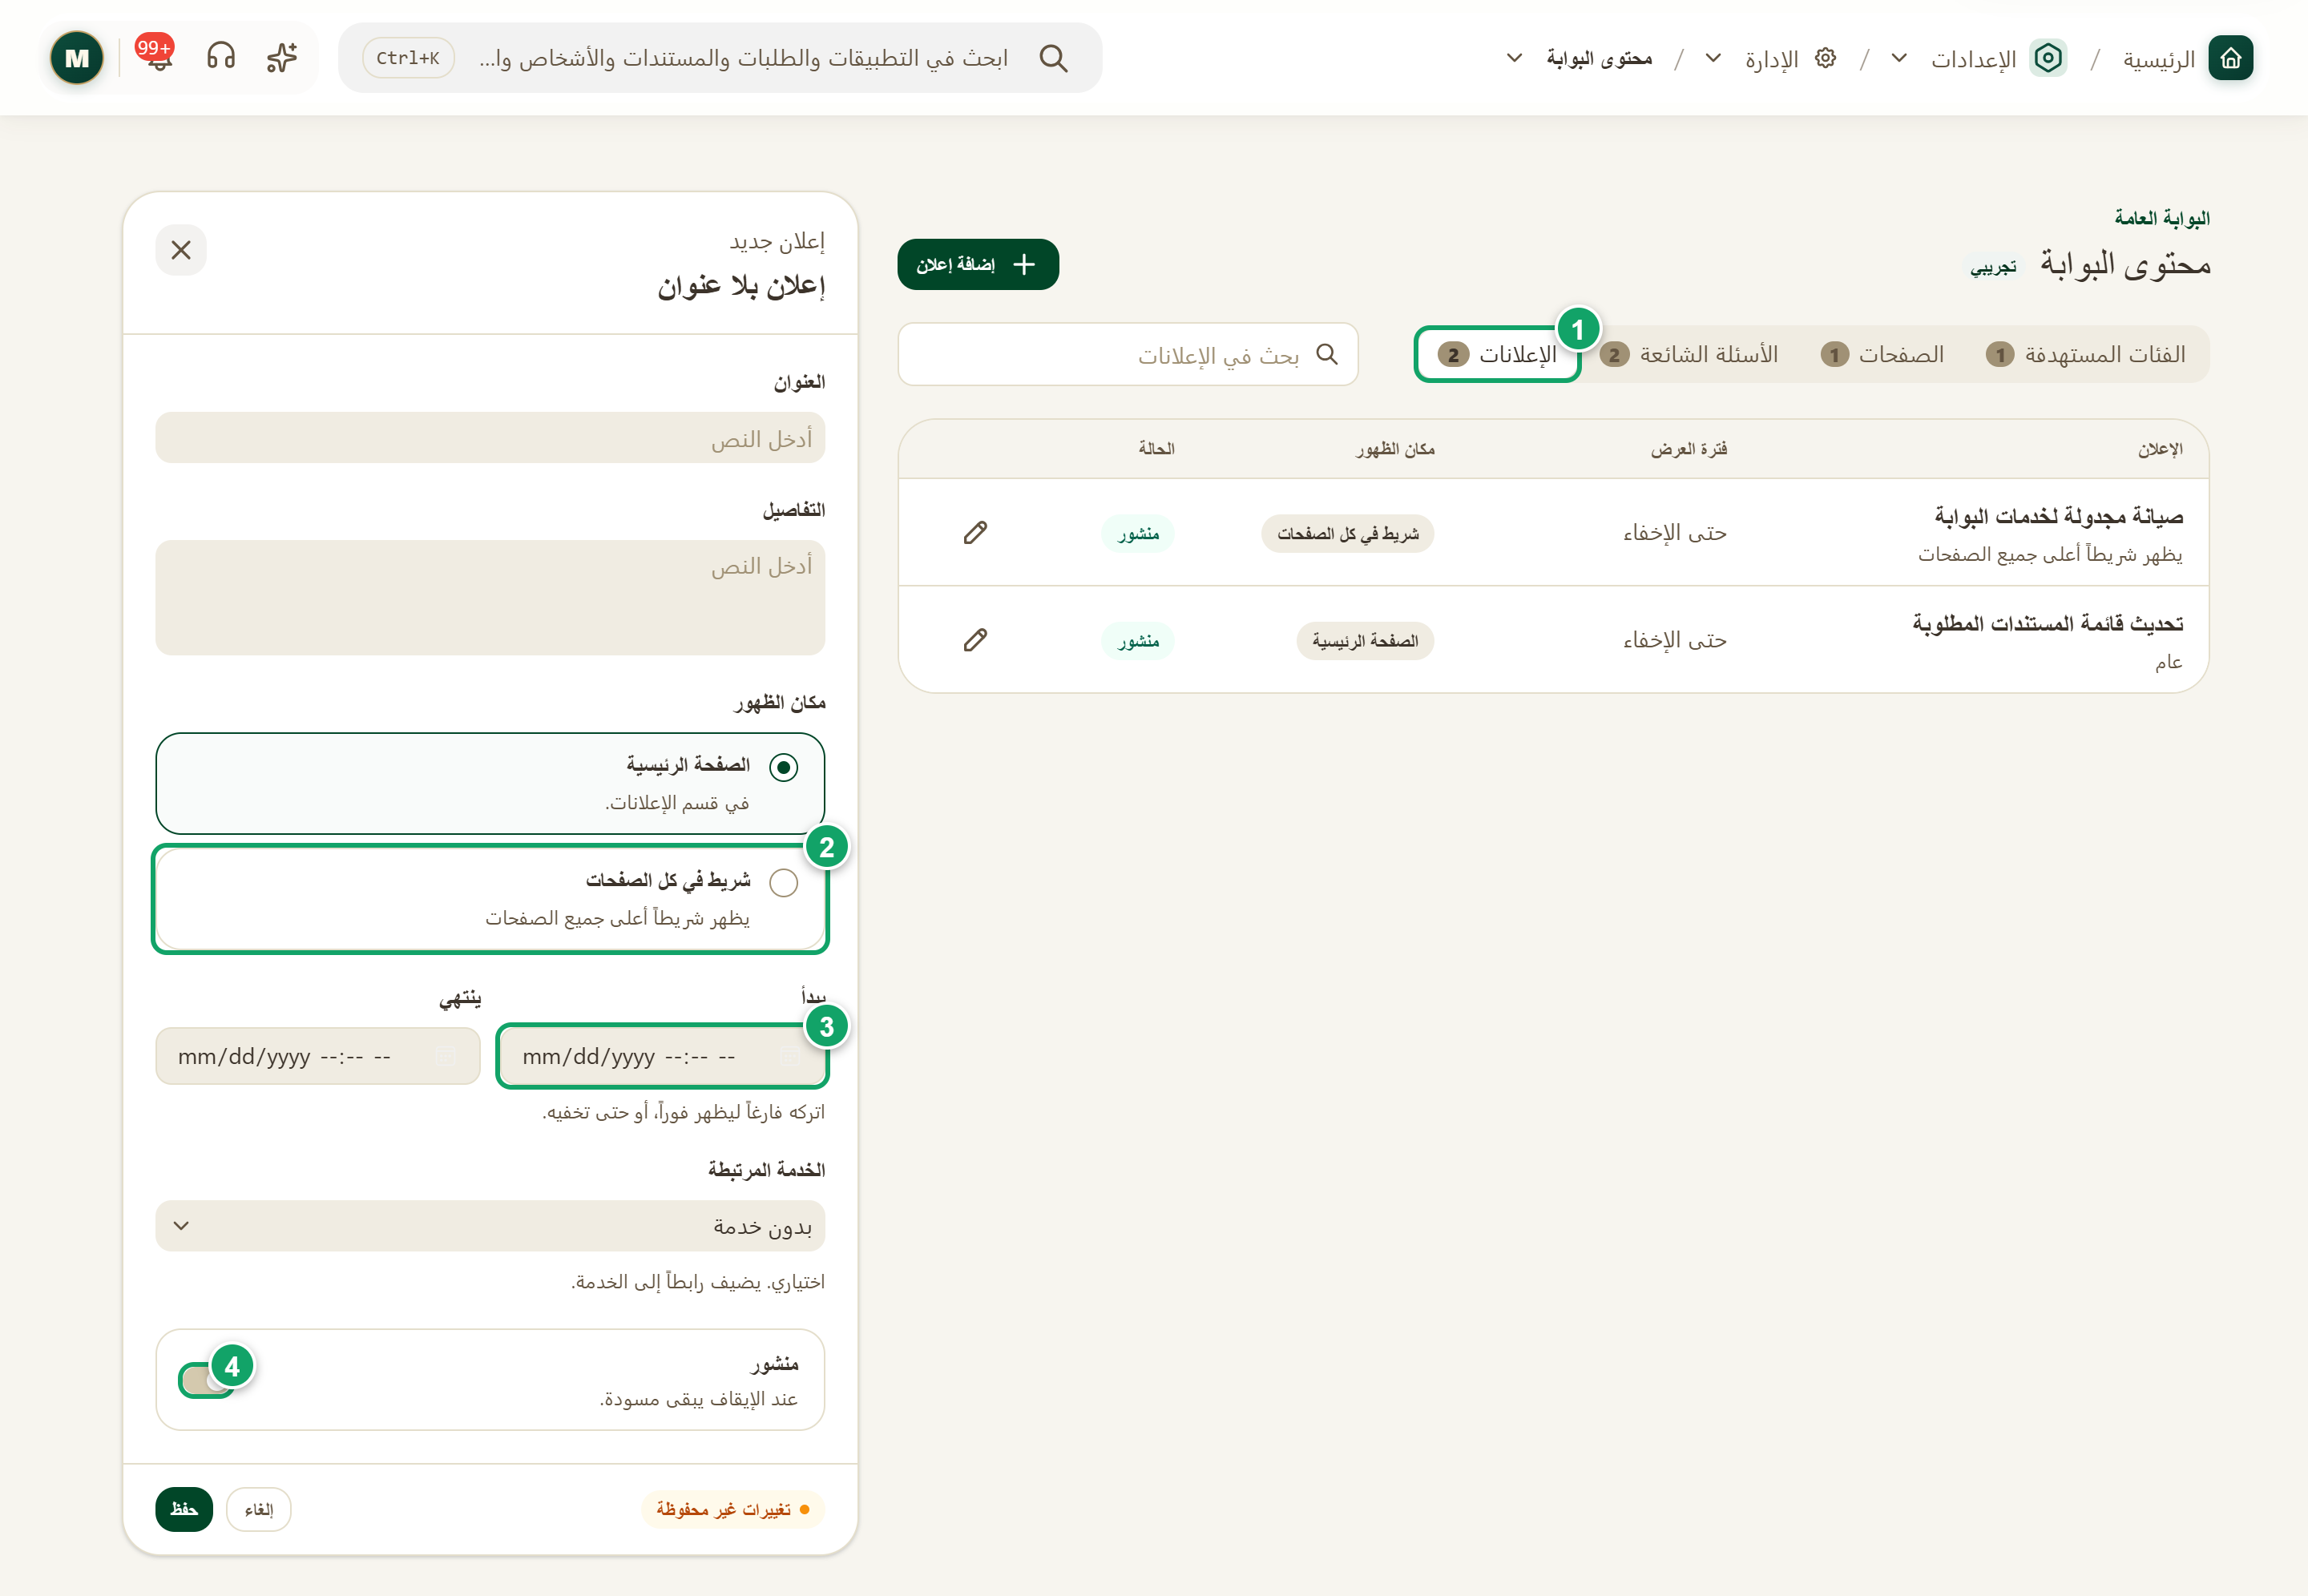
\includegraphics[width=0.95\linewidth,height=0.72\textheight,keepaspectratio]{figures/screens/ch08-portal-content-announcement-ar.png}
\caption{نموذج إعلان جديد}
\label{fig:settings-portal-content-announcement}
\shotnote{يُفتح النموذج بجوار الجدول دون مغادرة الصفحة، والنموذج الظاهر فارغ ولم يُحفظ. يبقى الإعلان الجديد مسودة حتى تشغّل مفتاح النشر. ① «الإعلانات». ② «شريط في كل الصفحات»: بديل لعرضه في قسم الإعلانات بالصفحة الرئيسية. ③ حقل «يبدأ»: اتركها فارغة ليظهر الإعلان فوراً، واترك «ينتهي» فارغة ليبقى حتى تخفيه. ④ مفتاح «منشور».}
\end{figure}

\begin{table}[H]
\centering
\caption{ماذا تسجل في محتوى البوابة؟}
\label{tab:settings-portal-content-fields}
\begin{tabularx}{\linewidth}{R{4.2cm} Y}
\rcHeaderRow
\thh{التبويب} & \thh{ما الذي تسجله؟}\\
«الفئات المستهدفة» & «العنوان» و«الوصف» و«الأيقونة»، ثم الخدمات المعروضة من «التطبيقات» و«الأقسام» و«خدمات إضافية»، وأخيراً «الترتيب»؛ فالرقم الأصغر يظهر أولاً.\\
«الصفحات» & «العنوان» و«الرابط» بأحرف لاتينية صغيرة وأرقام وشرطات، و«المحتوى»، و«ظاهرة في التذييل».\\
«الأسئلة الشائعة» & «السؤال» و«الإجابة» و«النطاق»: «البوابة كاملة» أو «تطبيق» أو «خدمات محددة».\\
«الإعلانات» & «العنوان» و«التفاصيل» و«مكان الظهور» و«يبدأ» و«ينتهي» و«الخدمة المرتبطة» و«منشور». وتعرض الحالة: «منشور» أو «مجدول» أو «منتهٍ» أو «مسودة».\\
\end{tabularx}
\end{table}

\begin{enumerate}
\item افتح «الإعدادات»، ثم «محتوى البوابة».
\item اختر نوع المحتوى من التبويبات، ثم اضغط زر الإضافة أو زر التعديل في صف قائم.
\item املأ النموذج، واكتب النصوص بكل لغة تريد أن يقرأها المتعامل.
\item اضغط «حفظ». إذا عدّلت ثم أغلقت النموذج، تسألك الصفحة قبل تجاهل التغييرات.
\item لحذف عنصر، افتحه واضغط «حذف» وأكّد؛ فلن يراه المتعاملون بعد ذلك.
\end{enumerate}

\textbf{تحقق:} يظهر العنصر في جدوله، ويزداد العدد بجوار اسم التبويب. افتح البوابة وتأكد من ظهوره في مكانه. وإذا لم تظهر الفئات أو الإعلانات، فراجع إخفاء قسمها في «أقسام الصفحة الرئيسية».

\clearpage
\section{حسابات المتعاملين}
\label{sec:settings-feature-applicant-profile}

ينشئ المتعامل حساباً واحداً يقدم به طلباته، حتى لا يكرر بياناته في كل طلب. تحدد هذه الصفحة البيانات التي يملؤها في ملفه الشخصي، ومتى تُطلب منه، وكيف يجري التأكد من صحتها. والتحقق هو التأكد من أن القيمة صحيحة، إما برمز يصل إلى هاتفه أو بريده، وإما بمراجعة موظف.

تعود إلى هذه الصفحة قبل نشر خدمات تحتاج إلى بيانات موثوقة، مثل رقم الهوية. يفتحها مالك المؤسسة ومن يحمل دور المسؤول. ويحتوي «ملف الشركة» على إعدادات المتعاملين الذين يمثلون شركات.

\begin{rcnote}[مثال: شركة الأفق]
تحتاج إحدى خدمات الأفق إلى رقم هوية موثوق، فيضيف مسؤول النظام الحقل عند ②، ويجعل الموظف يتحقق منه. ثم ينشئ عند ⑤ مستوى تحقق يتطلب هذا الحقل، ليشترطه في تلك الخدمة.
\end{rcnote}
\begin{figure}[H]
\centering
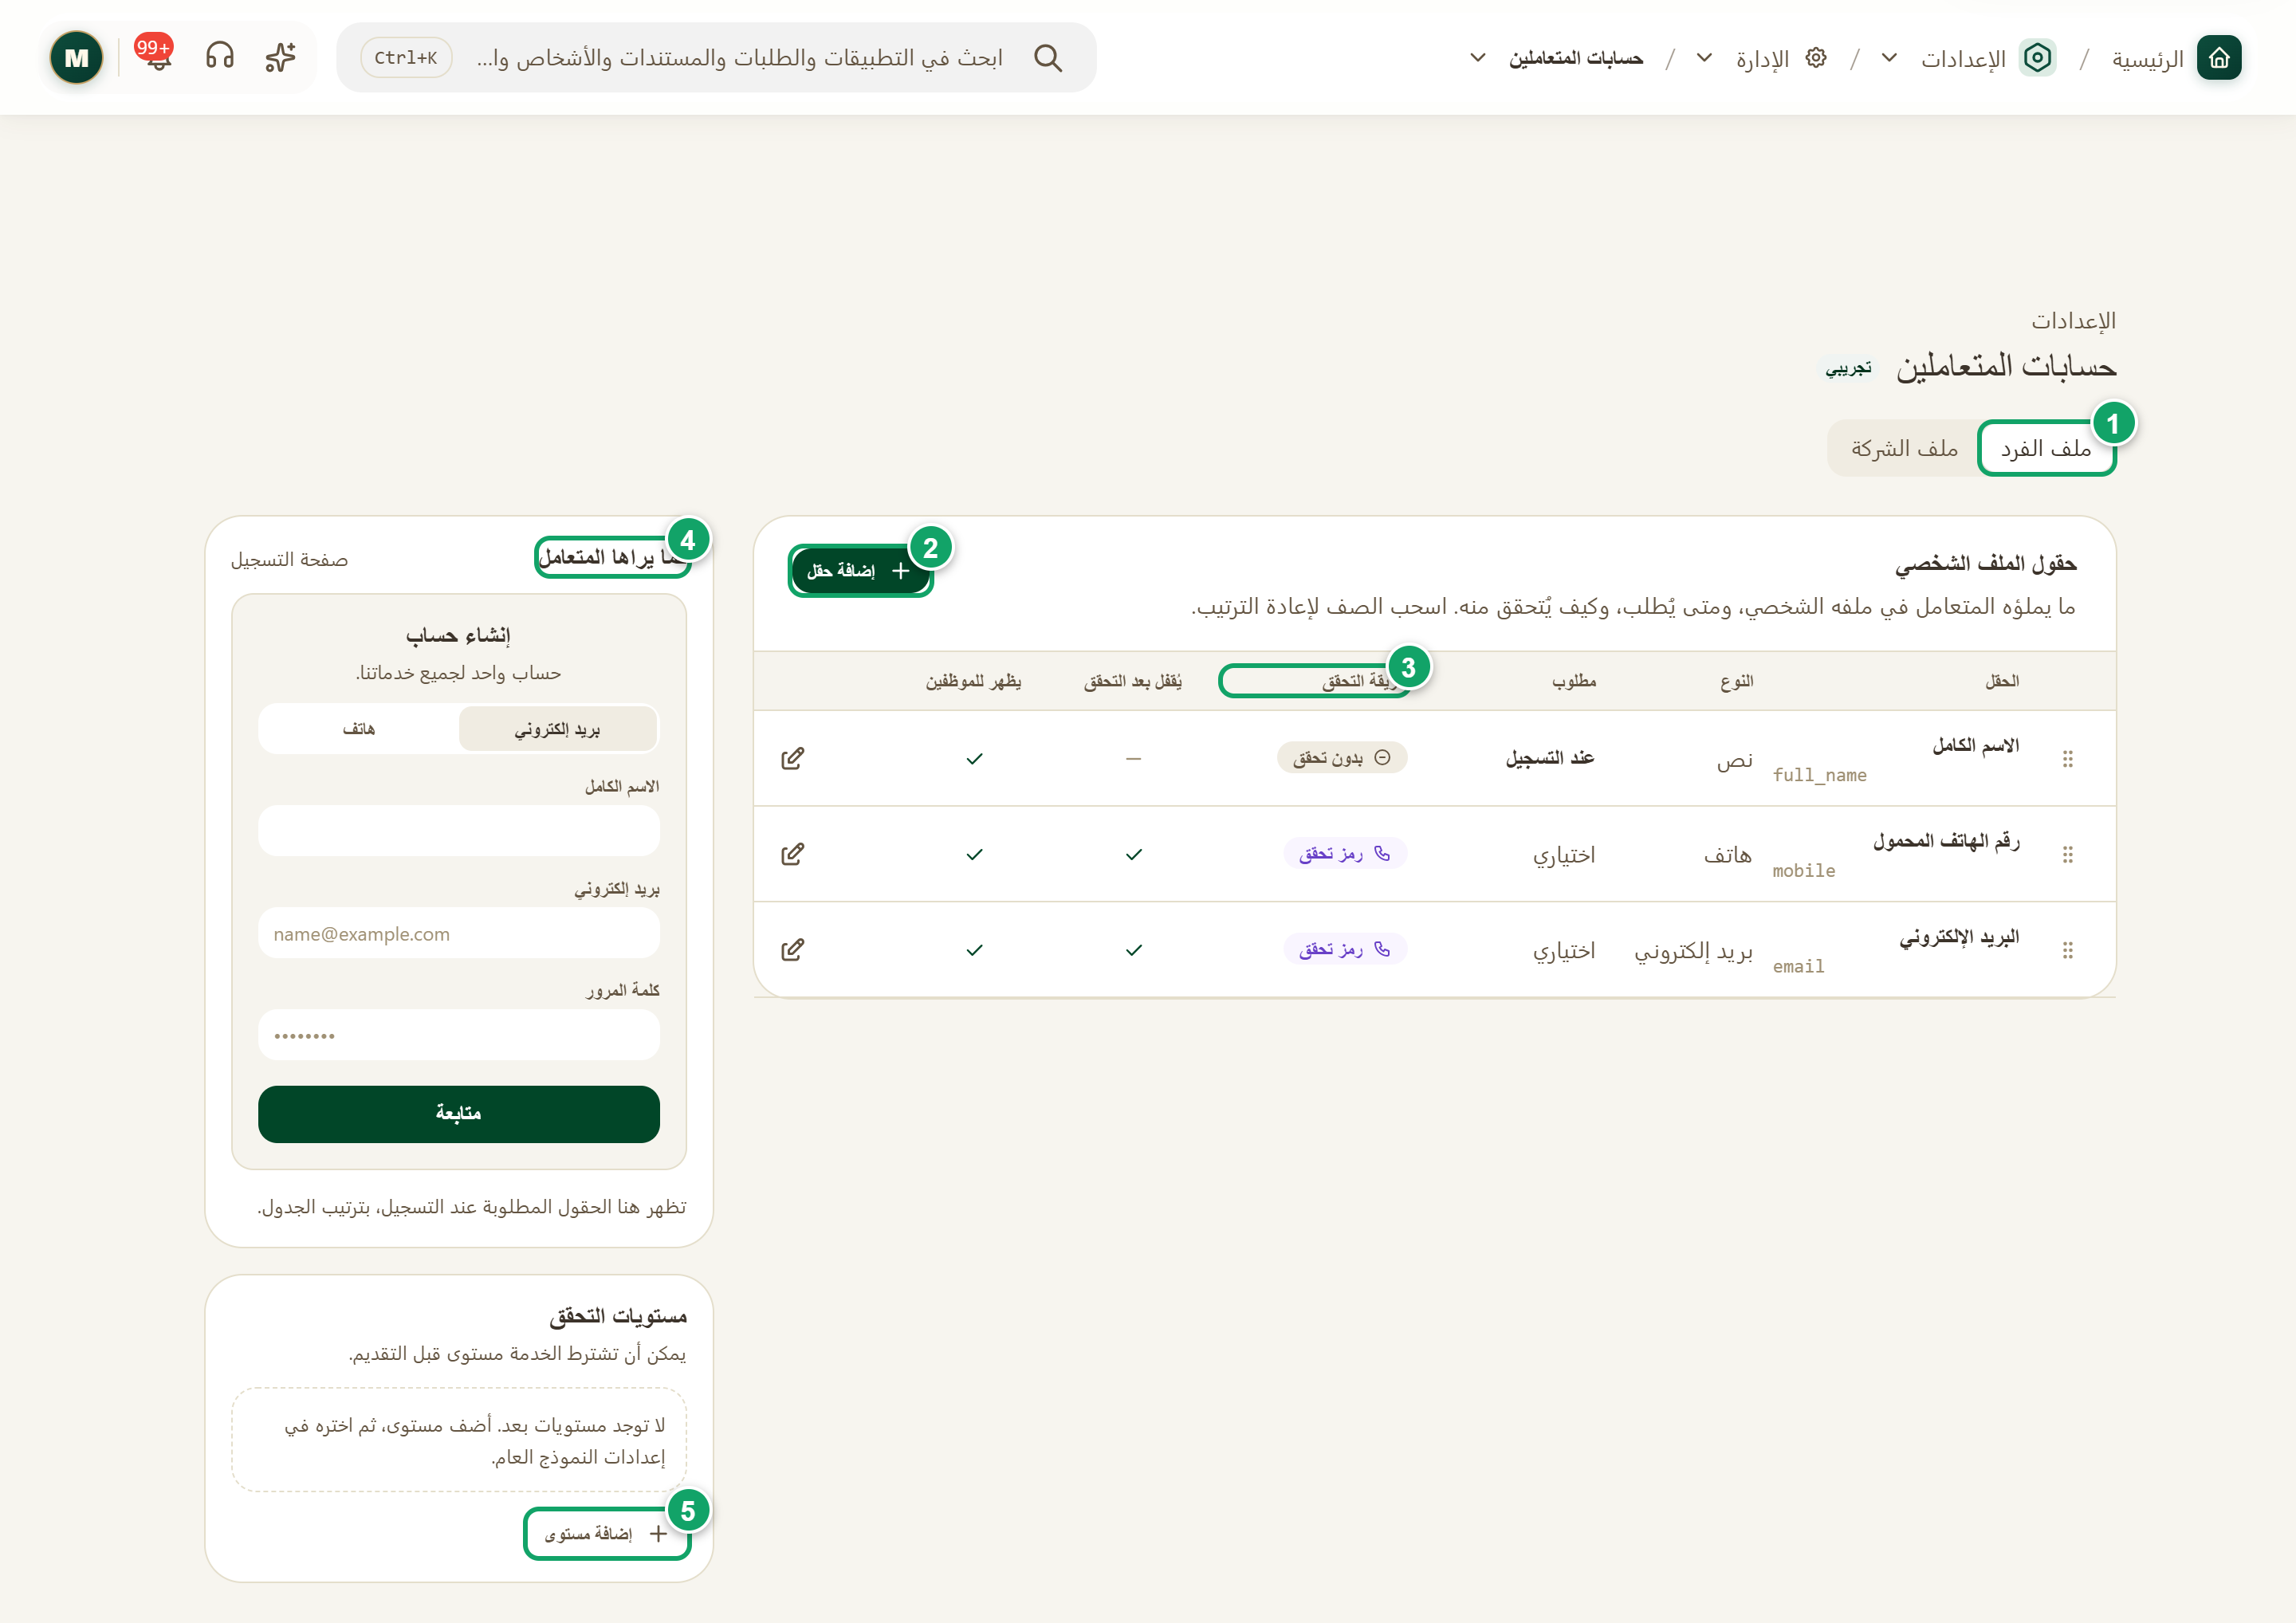
\includegraphics[width=0.95\linewidth,height=0.72\textheight,keepaspectratio]{figures/screens/ch08-applicant-profile-ar.png}
\caption{ملف الفرد}
\label{fig:settings-applicant-profile}
\shotnote{يجمع الجدول حقول الملف الشخصي، وتعرض البطاقة المجاورة أثرها على صفحة التسجيل. لم تُضف مؤسسة الاختبار مستويات تحقق بعد. ① «ملف الفرد». ② «إضافة حقل». ③ «طريقة التحقق»: تبين كيف تُؤكَّد قيمة كل حقل. ④ «كما يراها المتعامل»: معاينة صفحة التسجيل. ⑤ «إضافة مستوى».}
\end{figure}

\begin{figure}[H]
\centering
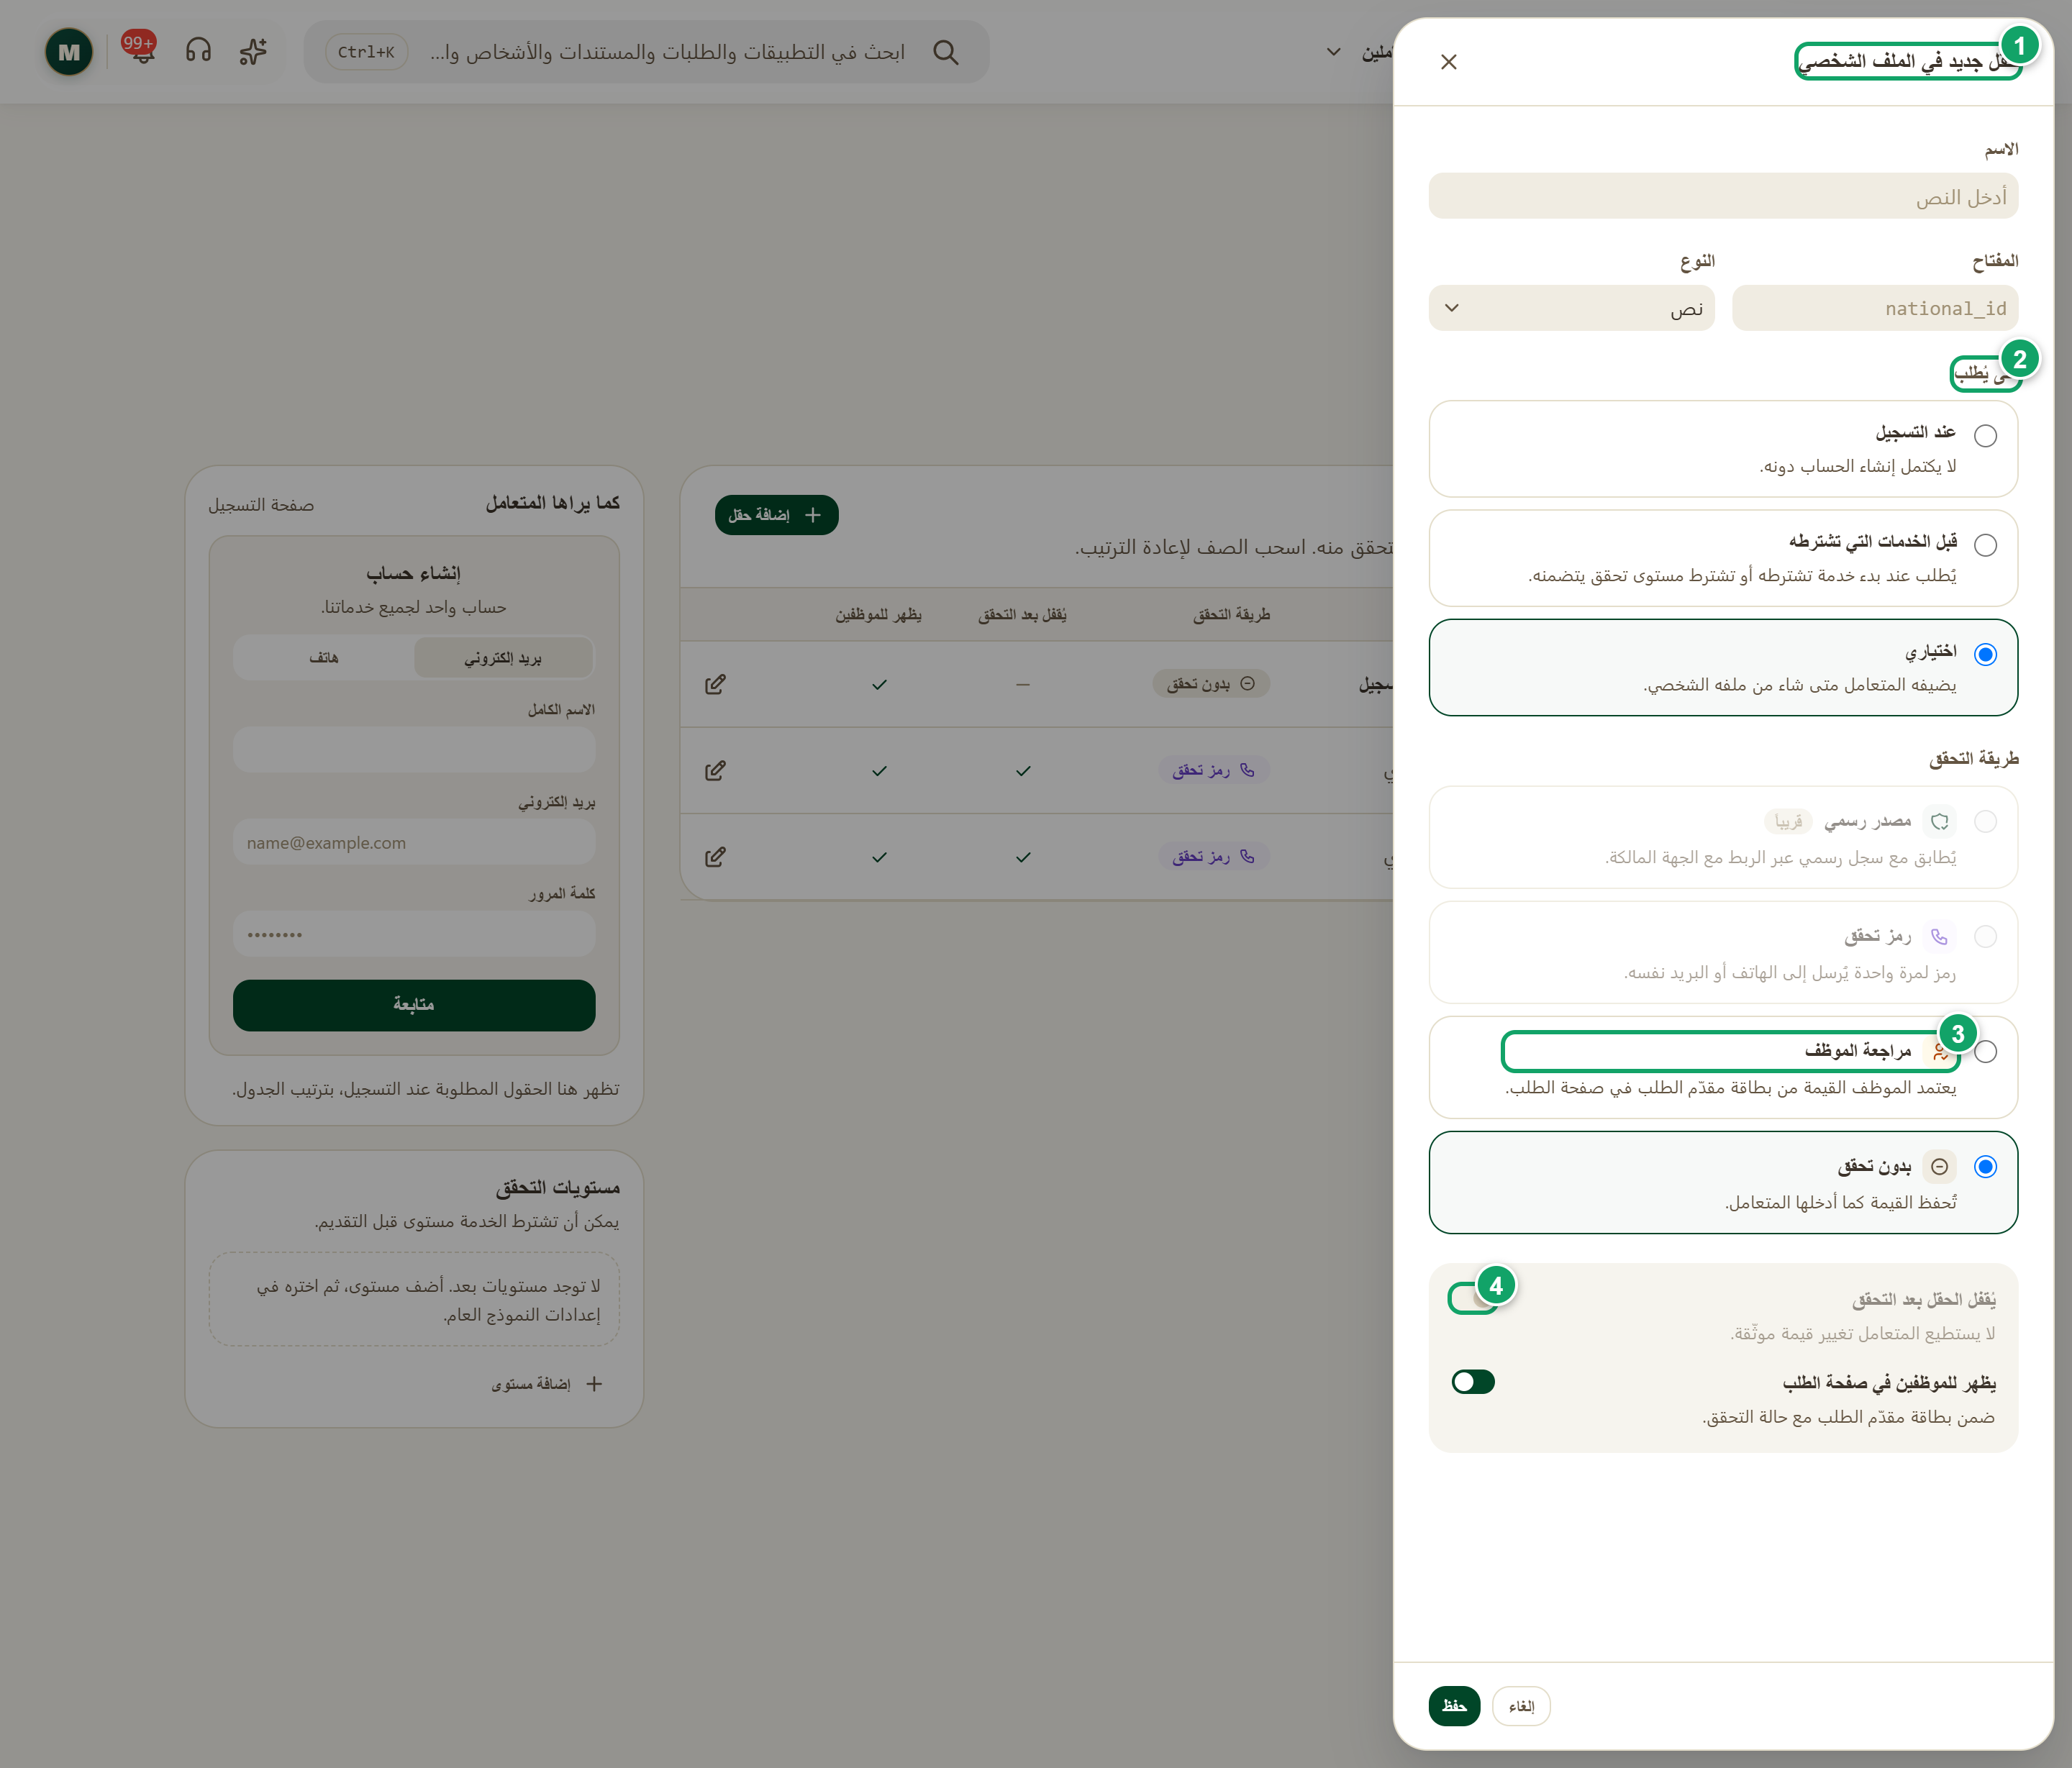
\includegraphics[width=0.95\linewidth,height=0.72\textheight,keepaspectratio]{figures/screens/ch08-applicant-profile-field-ar.png}
\caption{نموذج حقل جديد}
\label{fig:settings-applicant-profile-field}
\shotnote{يُفتح النموذج عند إضافة حقل أو تعديله، والصورة تعرضه فارغاً ولم يُحفظ. تظهر الخيارات غير المتاحة باهتة؛ فالحقول المخصصة لا تدعم إلا مراجعة الموظف أو عدم التحقق، وخيار «مصدر رسمي» قادم لاحقاً. ① عنوان النموذج. ② «متى يُطلب». ③ «مراجعة الموظف»: يعتمد الموظف القيمة من صفحة الطلب. ④ «يُقفل الحقل بعد التحقق»: يمنع المتعامل من تغيير قيمة موثّقة، ولا يعمل مع «بدون تحقق».}
\end{figure}

\begin{figure}[H]
\centering
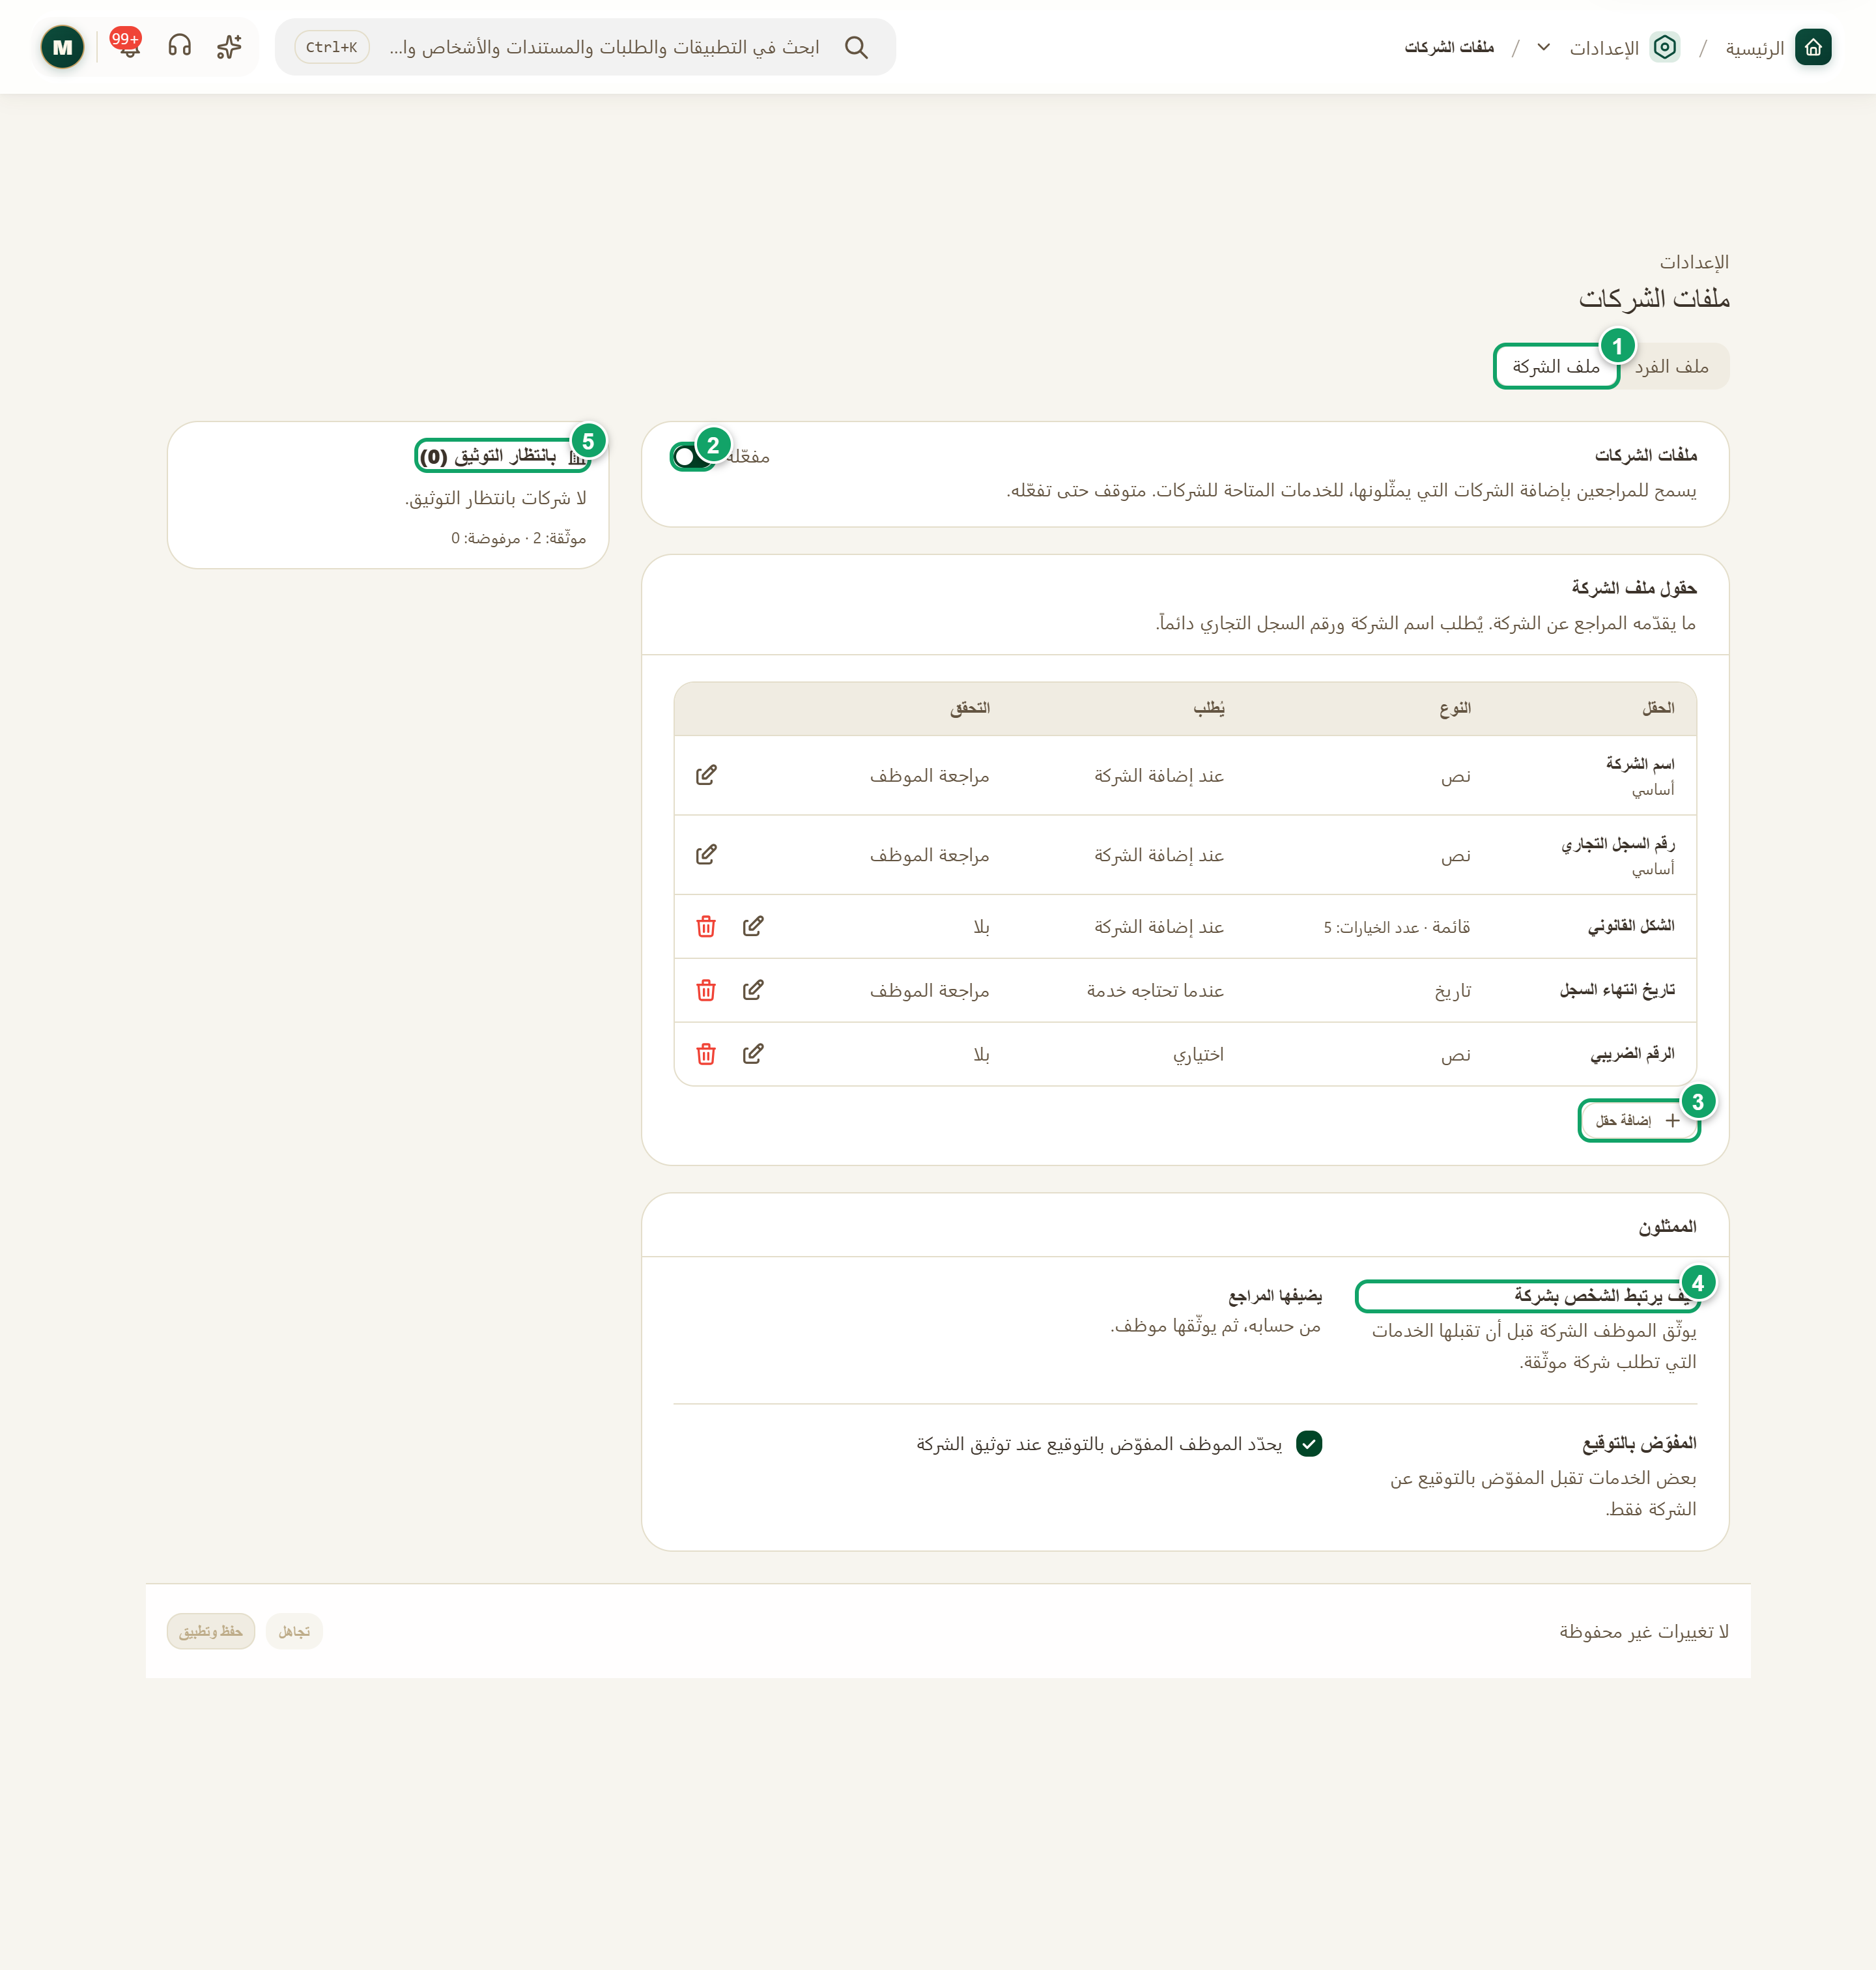
\includegraphics[width=0.95\linewidth,height=0.72\textheight,keepaspectratio]{figures/screens/ch08-applicant-company-ar.png}
\caption{ملف الشركة}
\label{fig:settings-applicant-company}
\shotnote{يخص هذا القسم المتعامل الذي يقدم باسم شركة يمثلها. يوثّق الموظف الشركة أولاً، أي يتأكد من صحة بياناتها، قبل أن تقبلها الخدمات التي تطلب شركة موثّقة. البيانات الظاهرة تخص مؤسسة الاختبار. ① «ملف الشركة». ② مفتاح تفعيل «ملفات الشركات»؛ وهي متوقفة حتى تفعّلها. ③ «إضافة حقل». ④ «كيف يرتبط الشخص بشركة». ⑤ «بانتظار التوثيق»: الشركات التي تنتظر مراجعة الموظف.}
\end{figure}

\begin{table}[H]
\centering
\caption{ماذا تسجل في حسابات المتعاملين؟}
\label{tab:settings-applicant-profile-fields}
\begin{tabularx}{\linewidth}{R{4.2cm} Y}
\rcHeaderRow
\thh{القسم} & \thh{ما الذي تسجله؟}\\
«حقول الملف الشخصي» & «الاسم» و«المفتاح» و«النوع»: نص أو رقم أو تاريخ أو قائمة. والمفتاح اسم تقني ثابت بأحرف إنجليزية، ولا يتغير بعد الإضافة.\\
«متى يُطلب» & «عند التسجيل»، أو «قبل الخدمات التي تشترطه»، أو «اختياري».\\
«طريقة التحقق» & «رمز تحقق» للهاتف والبريد فقط، و«مراجعة الموظف»، و«بدون تحقق».\\
خيارات إضافية & «يُقفل الحقل بعد التحقق» و«يظهر للموظفين في صفحة الطلب».\\
«مستويات التحقق» & «الاسم» و«الحقول التي يتطلبها المستوى». يجب أن يُملأ كل حقل منها، وأن يُوثَّق إن كانت له طريقة تحقق.\\
«ملف الشركة» & التفعيل، و«حقول ملف الشركة» بحد أقصى 20 حقلاً، وخيار تحديد «المفوّض بالتوقيع» عند التوثيق، ومراجعة الشركات المنتظرة بـ«توثيق» أو «رفض».\\
\end{tabularx}
\end{table}

\begin{enumerate}
\item افتح «الإعدادات»، ثم «حسابات المتعاملين».
\item اضغط «إضافة حقل»، واكتب الاسم والمفتاح واختر النوع.
\item حدد «متى يُطلب» و«طريقة التحقق»، ثم اضغط «حفظ».
\item اسحب صف الحقل لتغيير ترتيبه؛ يُحفظ الترتيب مباشرة.
\item اضغط «إضافة مستوى»، وسمّه واختر حقوله، ثم اضغط «حفظ». اختر المستوى بعد ذلك في إعدادات النموذج العام للخدمة.
\item إذا كنت تتعامل مع شركات، افتح «ملف الشركة» وفعّل «ملفات الشركات»، ثم اضغط «حفظ وتطبيق».
\end{enumerate}

\textbf{تحقق:} يظهر الحقل في الجدول، وإذا اخترت «عند التسجيل» يظهر أيضاً في «كما يراها المتعامل». انتبه إلى أن زر حذف المستوى ينفّذ الحذف فوراً دون سؤال. أما حذف حقل فيبقي القيم المحفوظة، لكنها لا تظهر ولا تُطلب بعد ذلك.

\clearpage
\section{الرسائل}
\label{sec:settings-feature-messages}

تحدد هذه الصفحة ما يُبلَّغ به المتعاملون والأطراف الخارجية، وعبر أي قناة، وتحفظ سجلاً بكل ما أُرسل. والقناة هي وسيلة الوصول: رسالة نصية، أو واتساب، أو بريد إلكتروني، أو إشعار داخل البوابة. والمتغير خانة داخل النص، مثل «رقم الطلب»، يستبدلها النظام بالقيمة الفعلية عند الإرسال.

استخدم هذه الصفحة عند إطلاق خدمة جديدة، أو عند تغيير نص رسالة أو قاعدة إرسال، أو لمعرفة سبب عدم وصول رسالة. يفتحها مالك المؤسسة ومن يحمل دور المسؤول. وقد يمنح الدور عضواً آخر إدارة قوالب المتابعة أو الاطلاع على السجل فقط، فلا يرى إلا ما يخصه.

\begin{rcnote}[مثال: شركة الأفق]
يراجع مسؤول النظام حدث «مطلوب منك إجراء» عند ②، ثم يفتح قناة البريد عند ③ ويعدّل النص ويحفظه عند ⑤. وعندما تسأله سارة الخطيب لماذا لم يصل بريد إلى متعامل، يفتح «سجل الإرسال» ويقرأ حالة الرسالة.
\end{rcnote}
\begin{figure}[H]
\centering
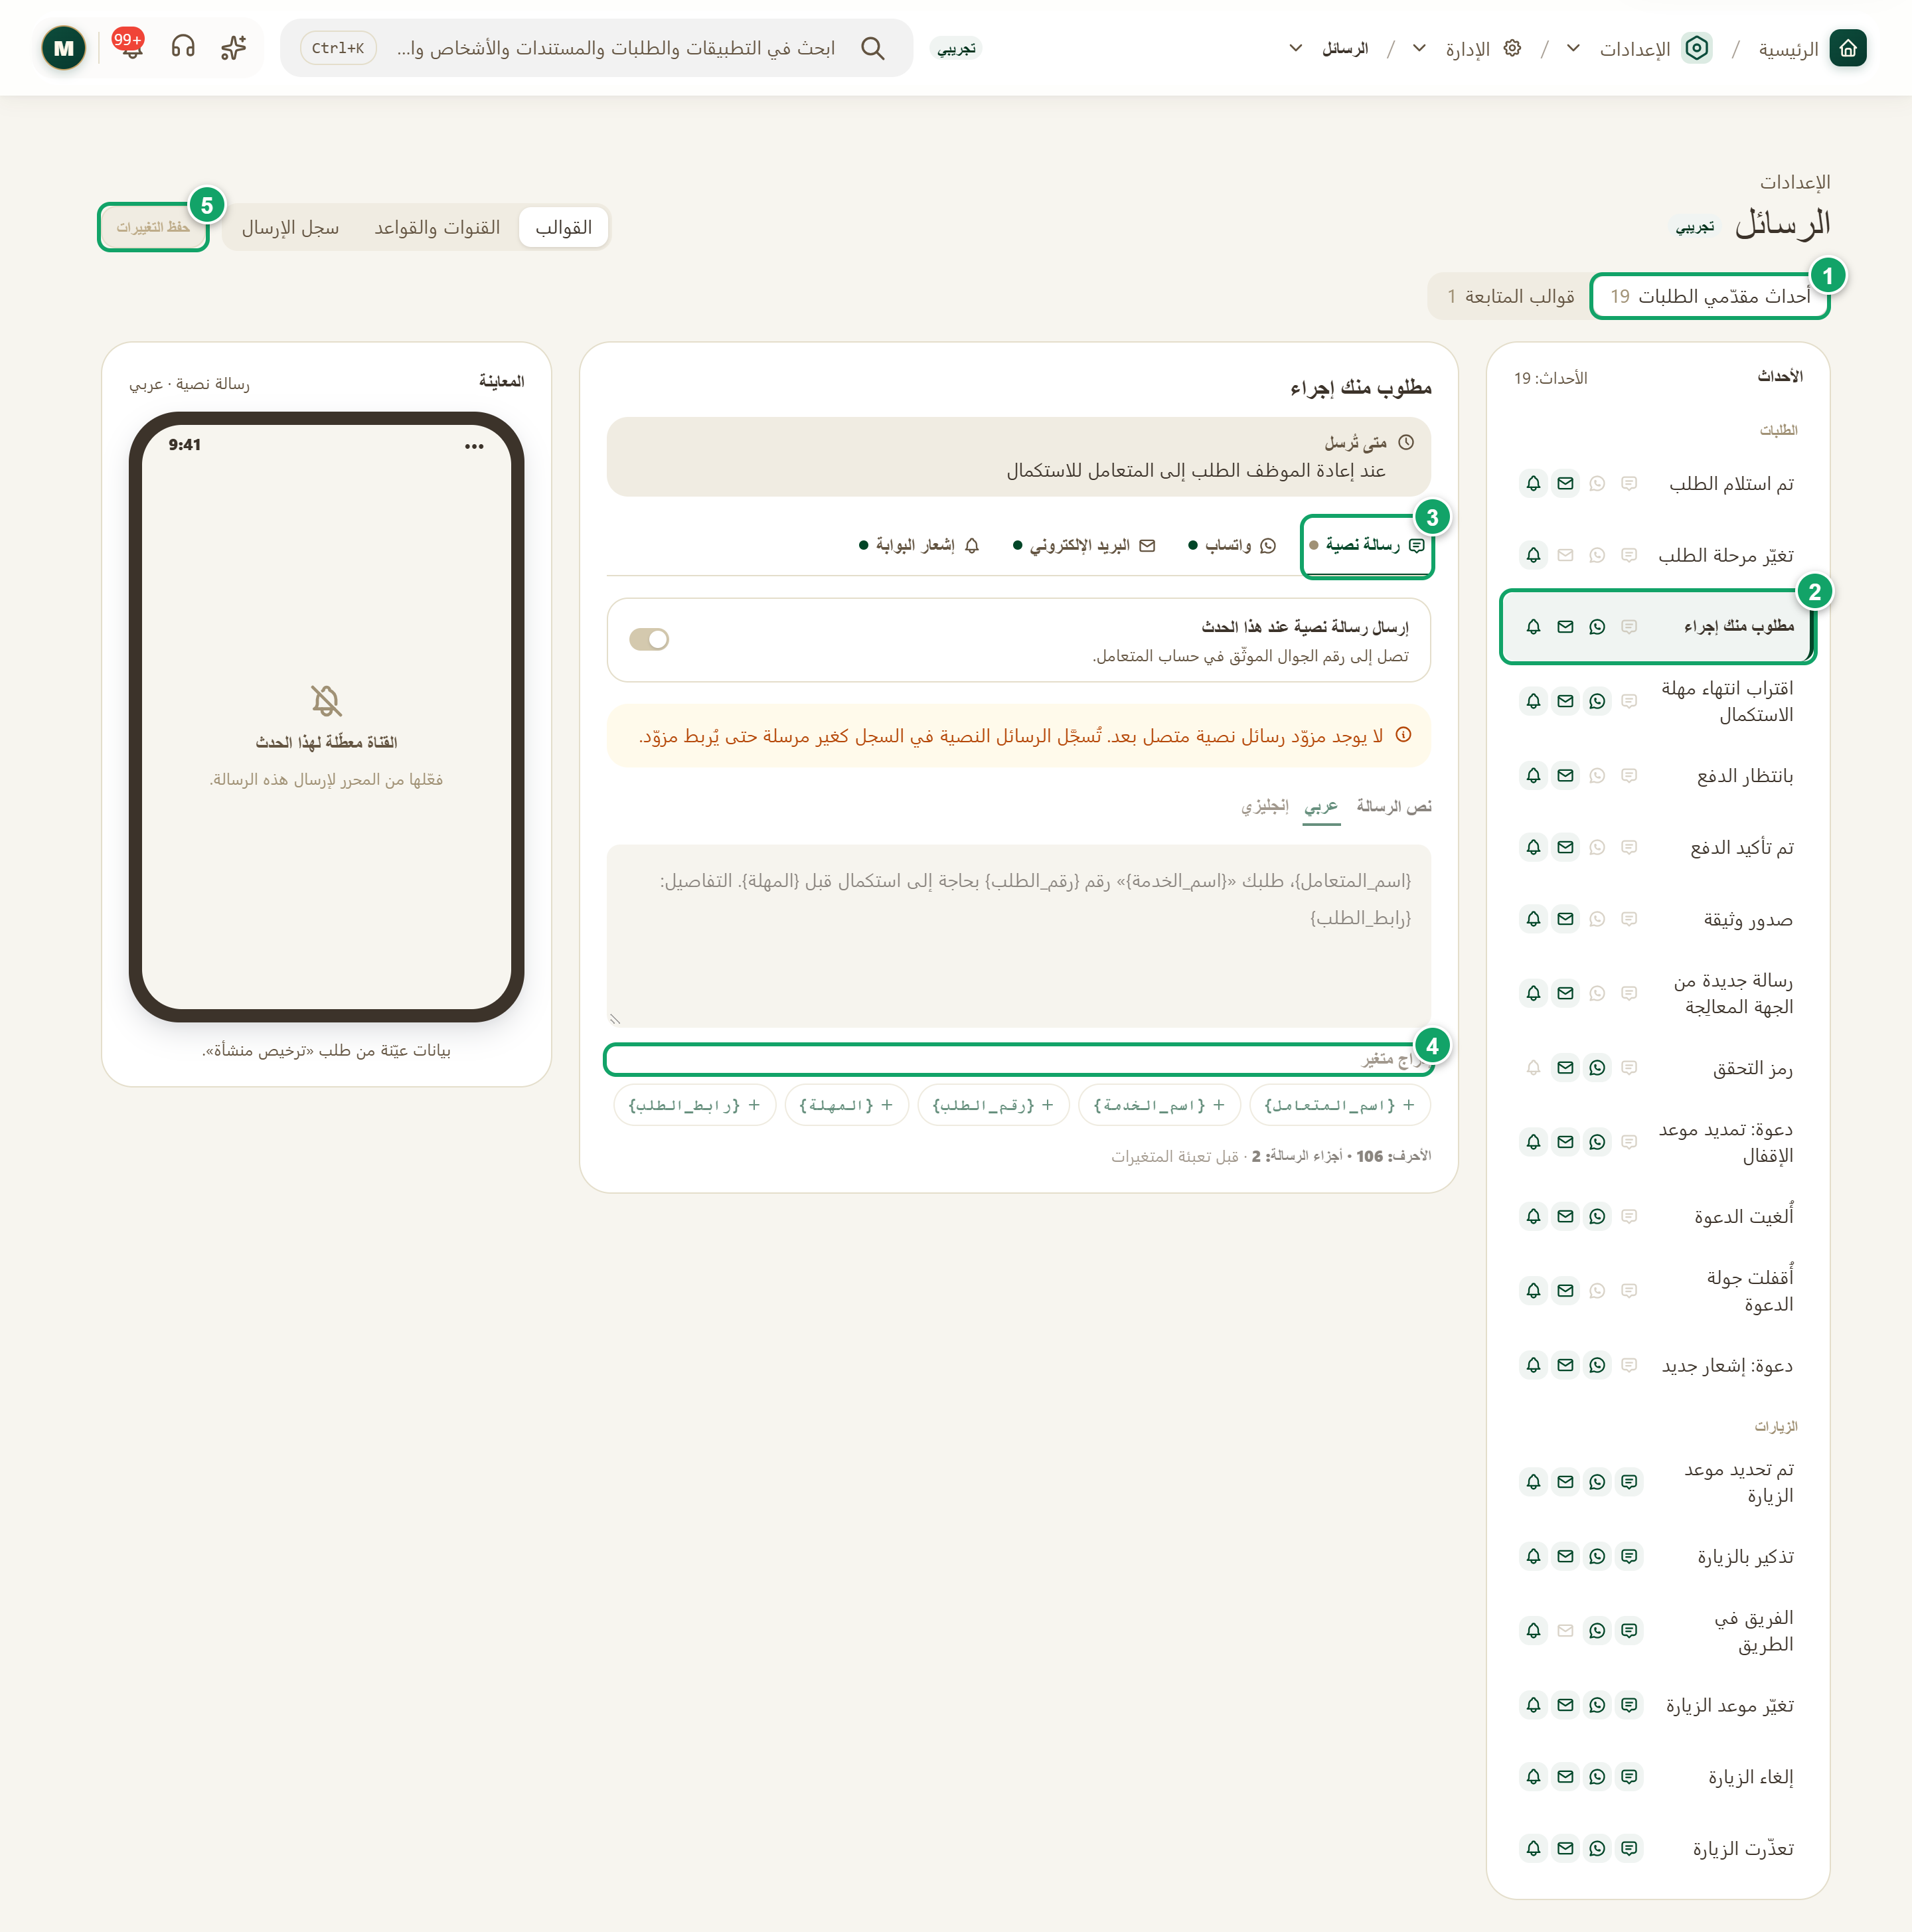
\includegraphics[width=0.95\linewidth,height=0.72\textheight,keepaspectratio]{figures/screens/ch08-messages-templates-ar.png}
\caption{أحداث مقدّمي الطلبات}
\label{fig:settings-messages-templates}
\shotnote{الحدث هو ما يدفع النظام إلى إرسال الرسالة، مثل استلام الطلب أو تغيّر موعد الزيارة. تعرض القائمة الأحداث التسعة عشر، ويبين كل صف قنواته المفعّلة، بينما تعرض المعاينة شكل الرسالة. ① «أحداث مقدّمي الطلبات». ② الحدث المختار. ③ القناة المختارة. ④ «إدراج متغير»: يضع قيمة متغيرة داخل النص. ⑤ «حفظ التغييرات».}
\end{figure}

\begin{figure}[H]
\centering
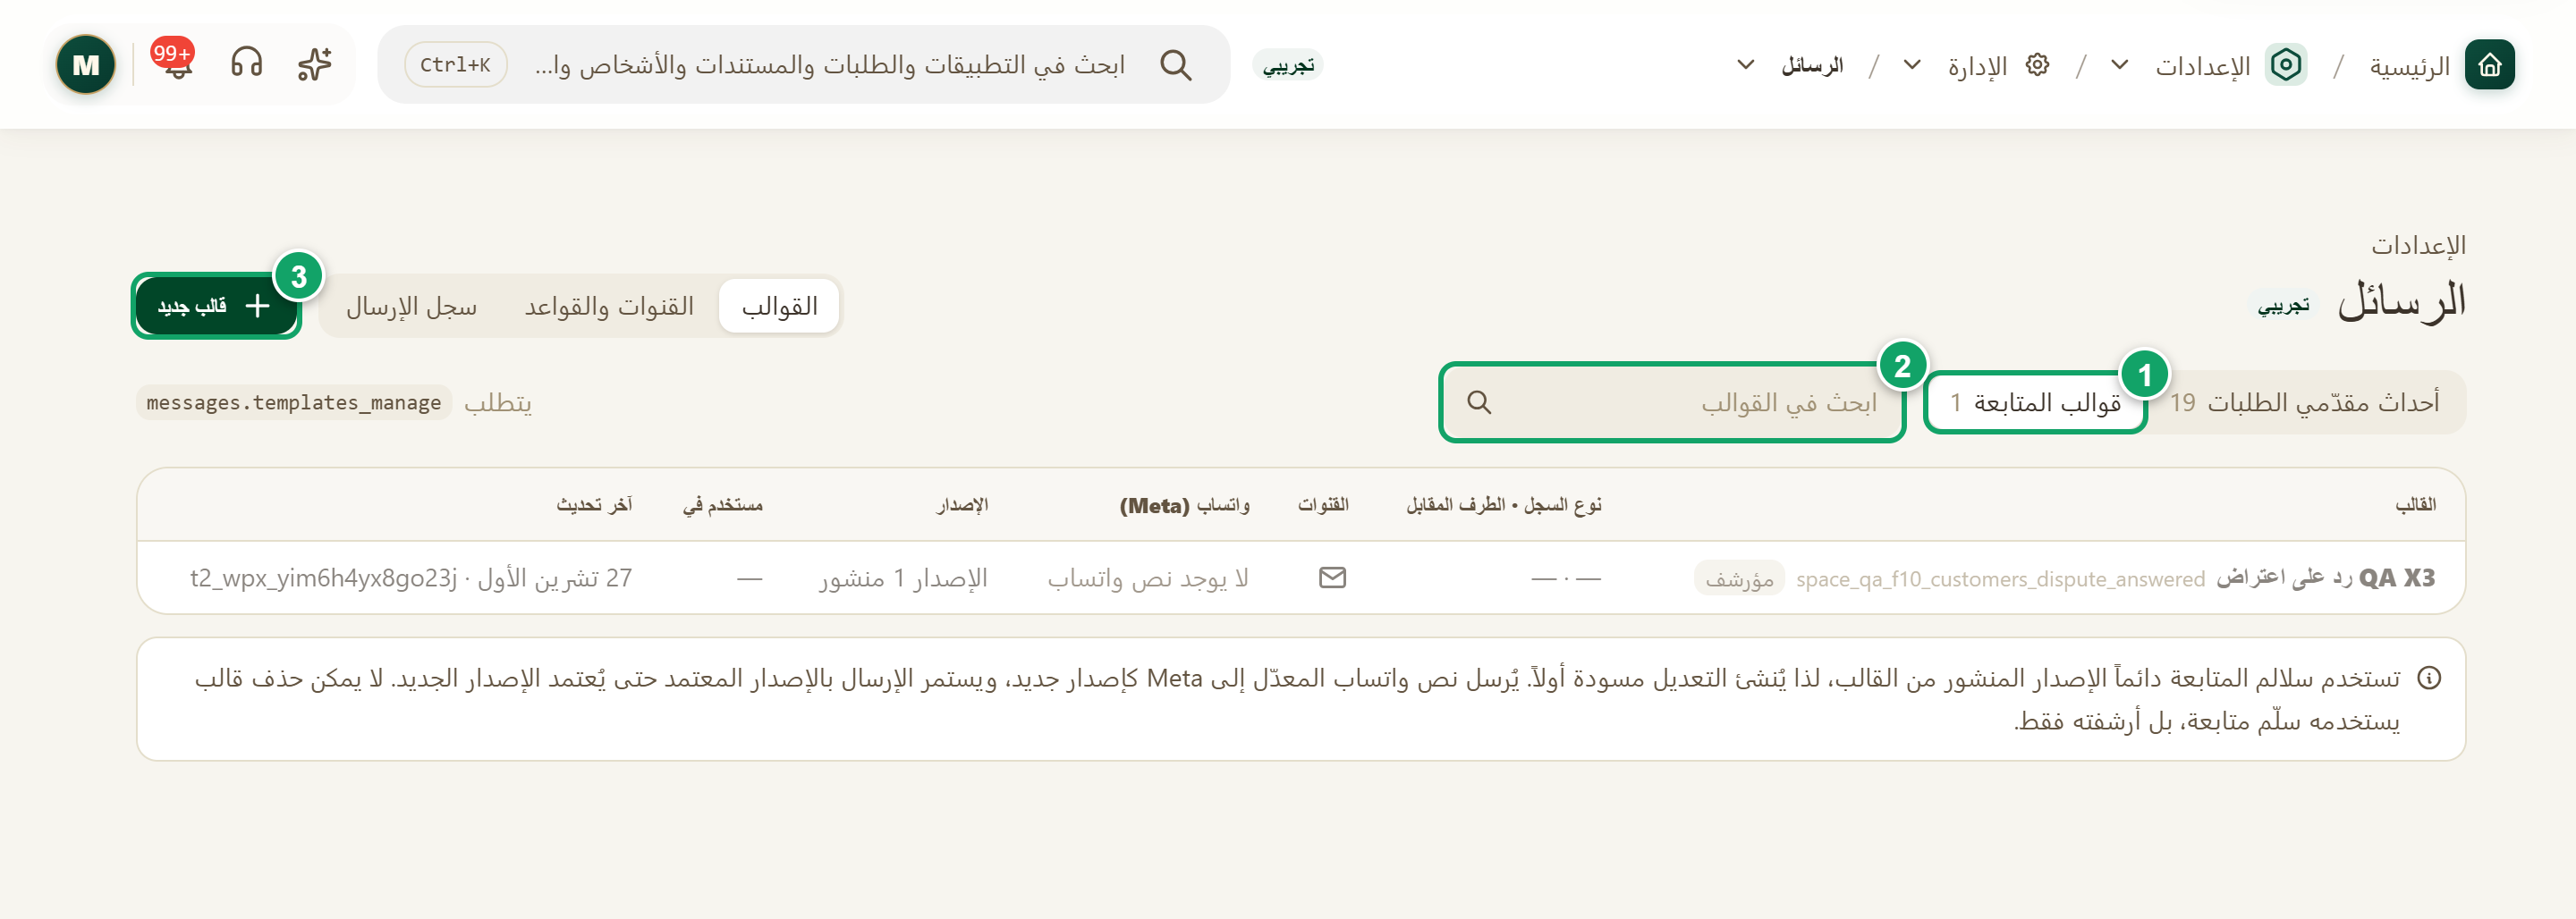
\includegraphics[width=0.95\linewidth,height=0.72\textheight,keepaspectratio]{figures/screens/ch08-messages-followup-ar.png}
\caption{قوالب المتابعة}
\label{fig:settings-messages-followup}
\shotnote{قالب المتابعة رسالة ترسلها خطوة في سلّم المتابعة، وهو تسلسل تذكيرات تتابع طرفاً حتى يتم المطلوب، كتذكير عميل بفاتورة مستحقة. تُرسل دائماً النسخة المنشورة، فيبدأ كل تعديل مسودة. ① «قوالب المتابعة». ② حقل البحث. ③ «قالب جديد».}
\end{figure}

\begin{figure}[H]
\centering
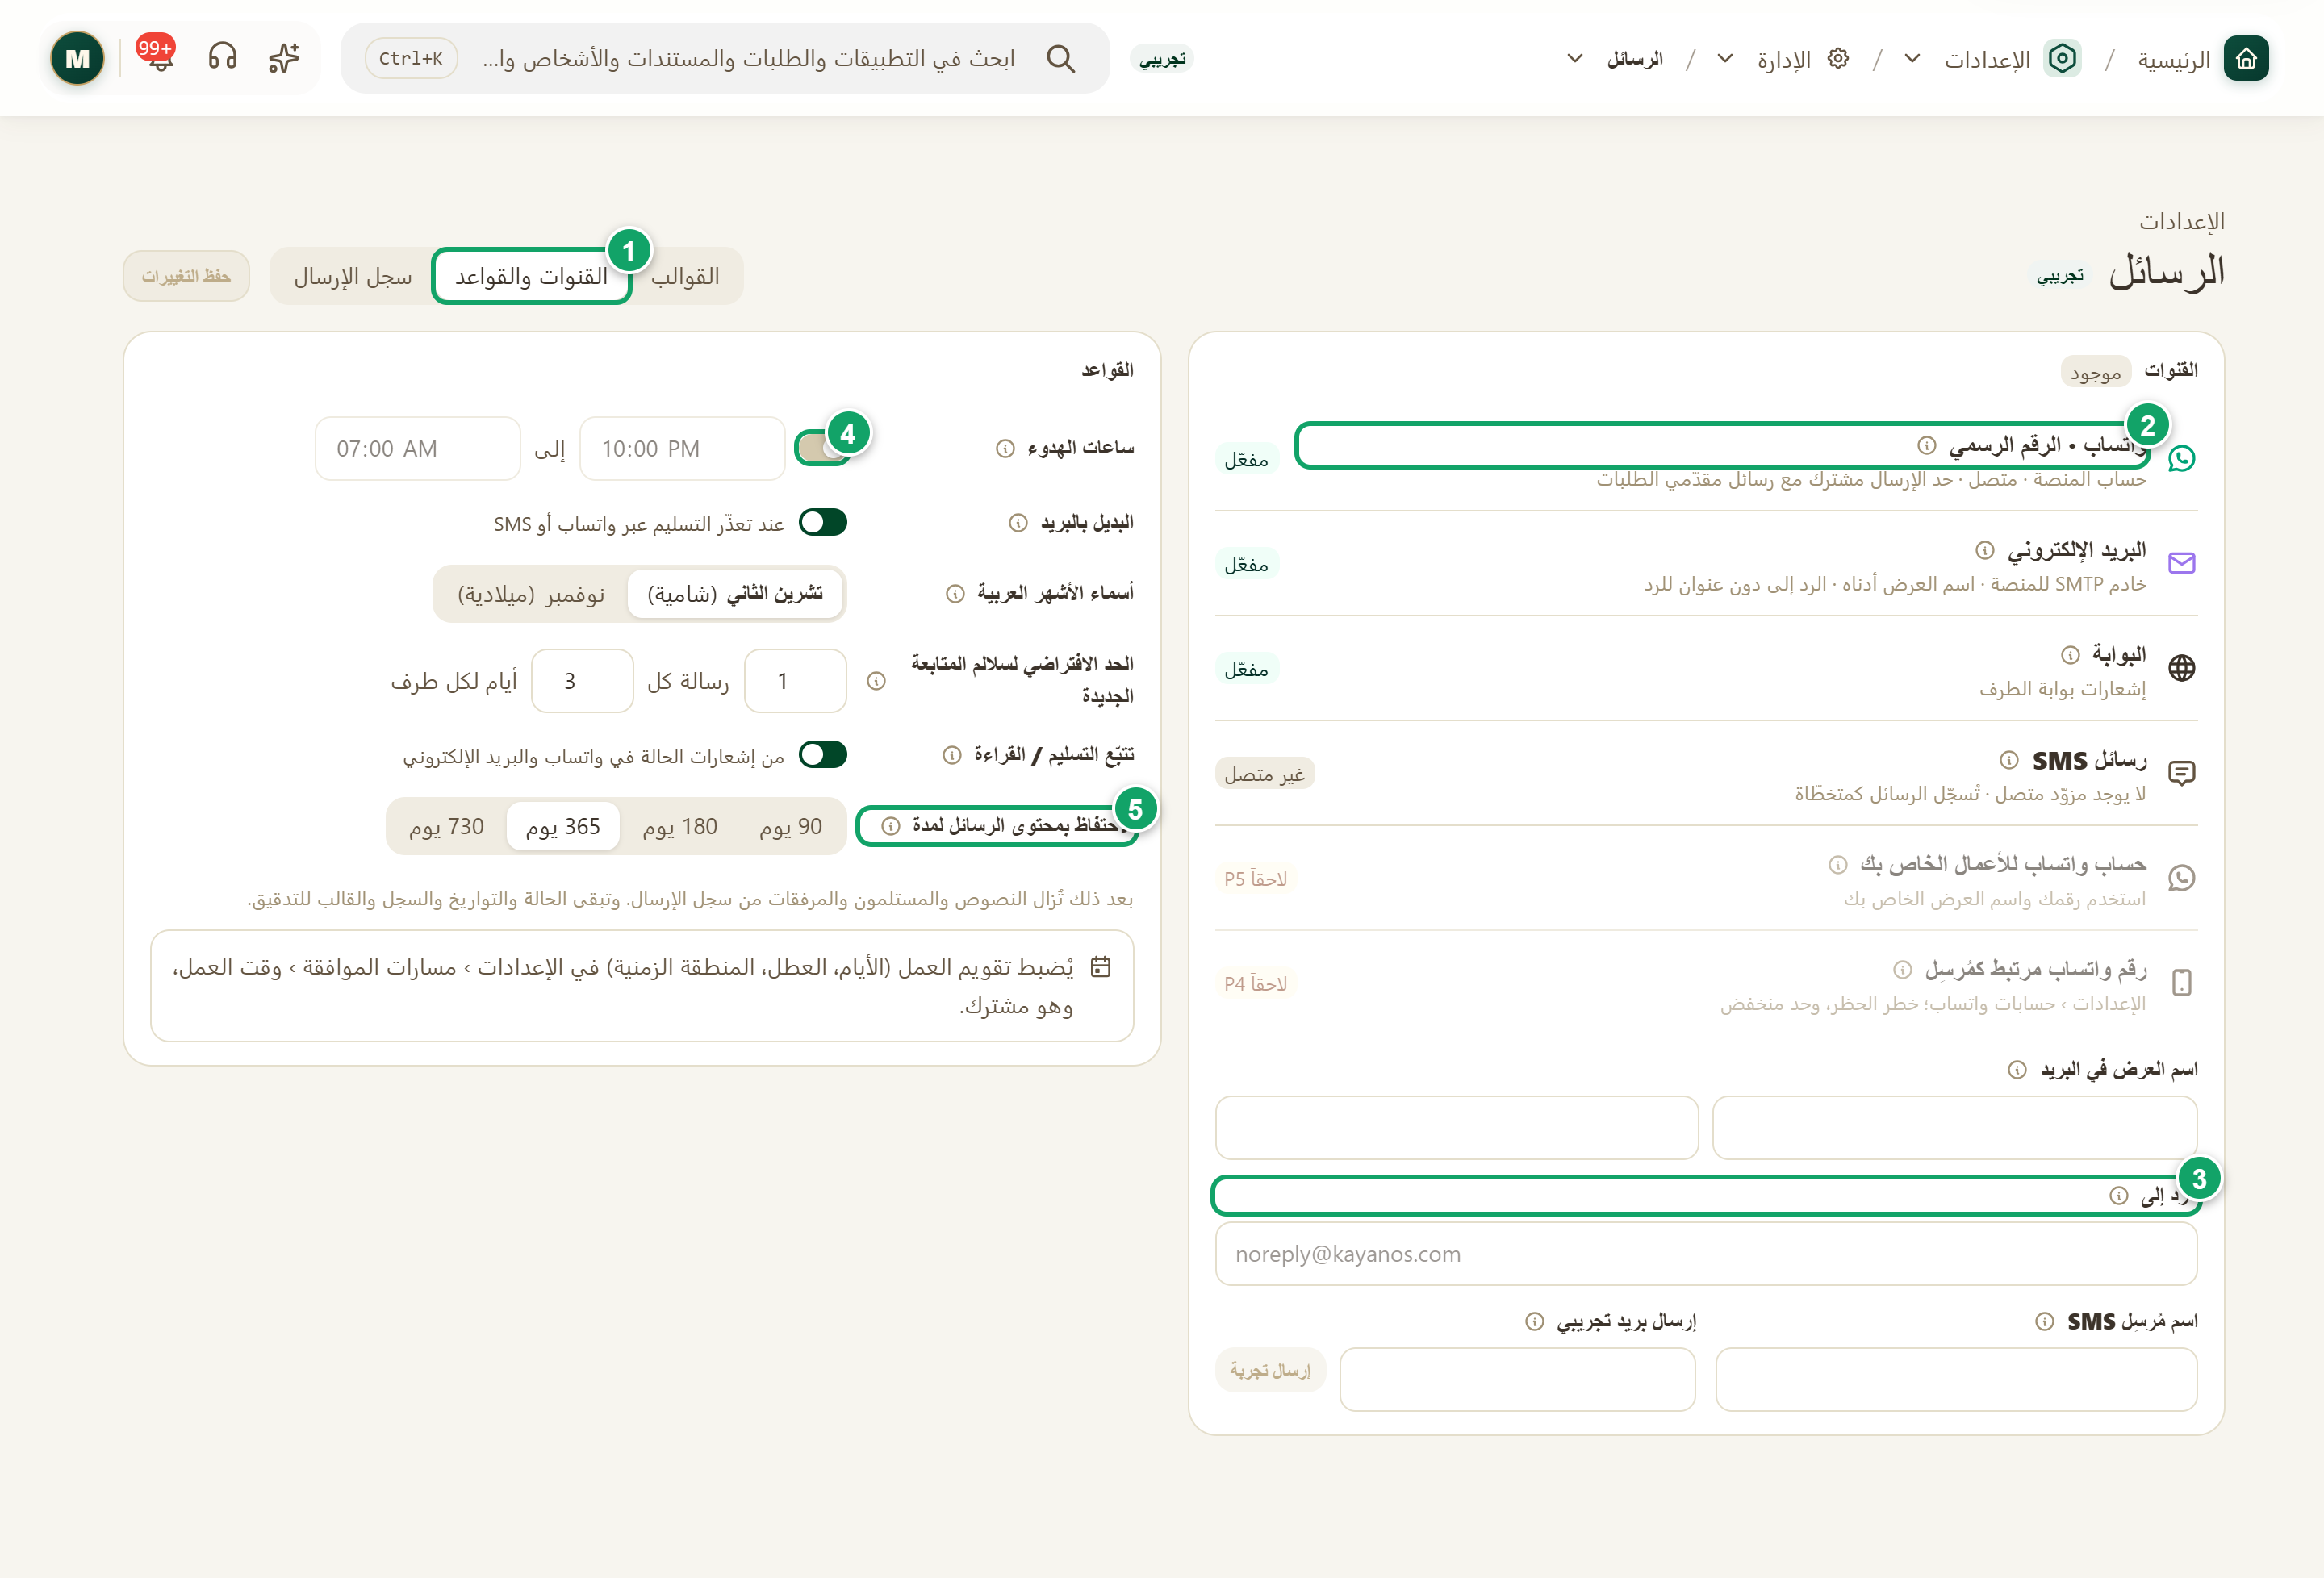
\includegraphics[width=0.95\linewidth,height=0.72\textheight,keepaspectratio]{figures/screens/ch08-messages-channels-ar.png}
\caption{القنوات والقواعد}
\label{fig:settings-messages-channels}
\shotnote{تجمع هذه الصفحة حالة القنوات والقواعد التي تسري على الرسائل. في مؤسسة الاختبار لا يوجد مزوّد للرسائل النصية، لذلك تُسجَّل هذه الرسائل بحالة «متخطّى» ولا تصل إلى أحد. ① «القنوات والقواعد». ② «واتساب · الرقم الرسمي»: الرقم الذي تُرسل منه هذه الرسائل. ③ «الرد إلى»: استخدم صندوقاً يقرؤه أحد، فإذا تركته فارغاً فلن تصل الردود. ④ مفتاح «ساعات الهدوء»: تنتظر الرسائل المستحقة خلالها حتى تنتهي. ⑤ «الاحتفاظ بمحتوى الرسائل لمدة».}
\end{figure}

\begin{figure}[H]
\centering
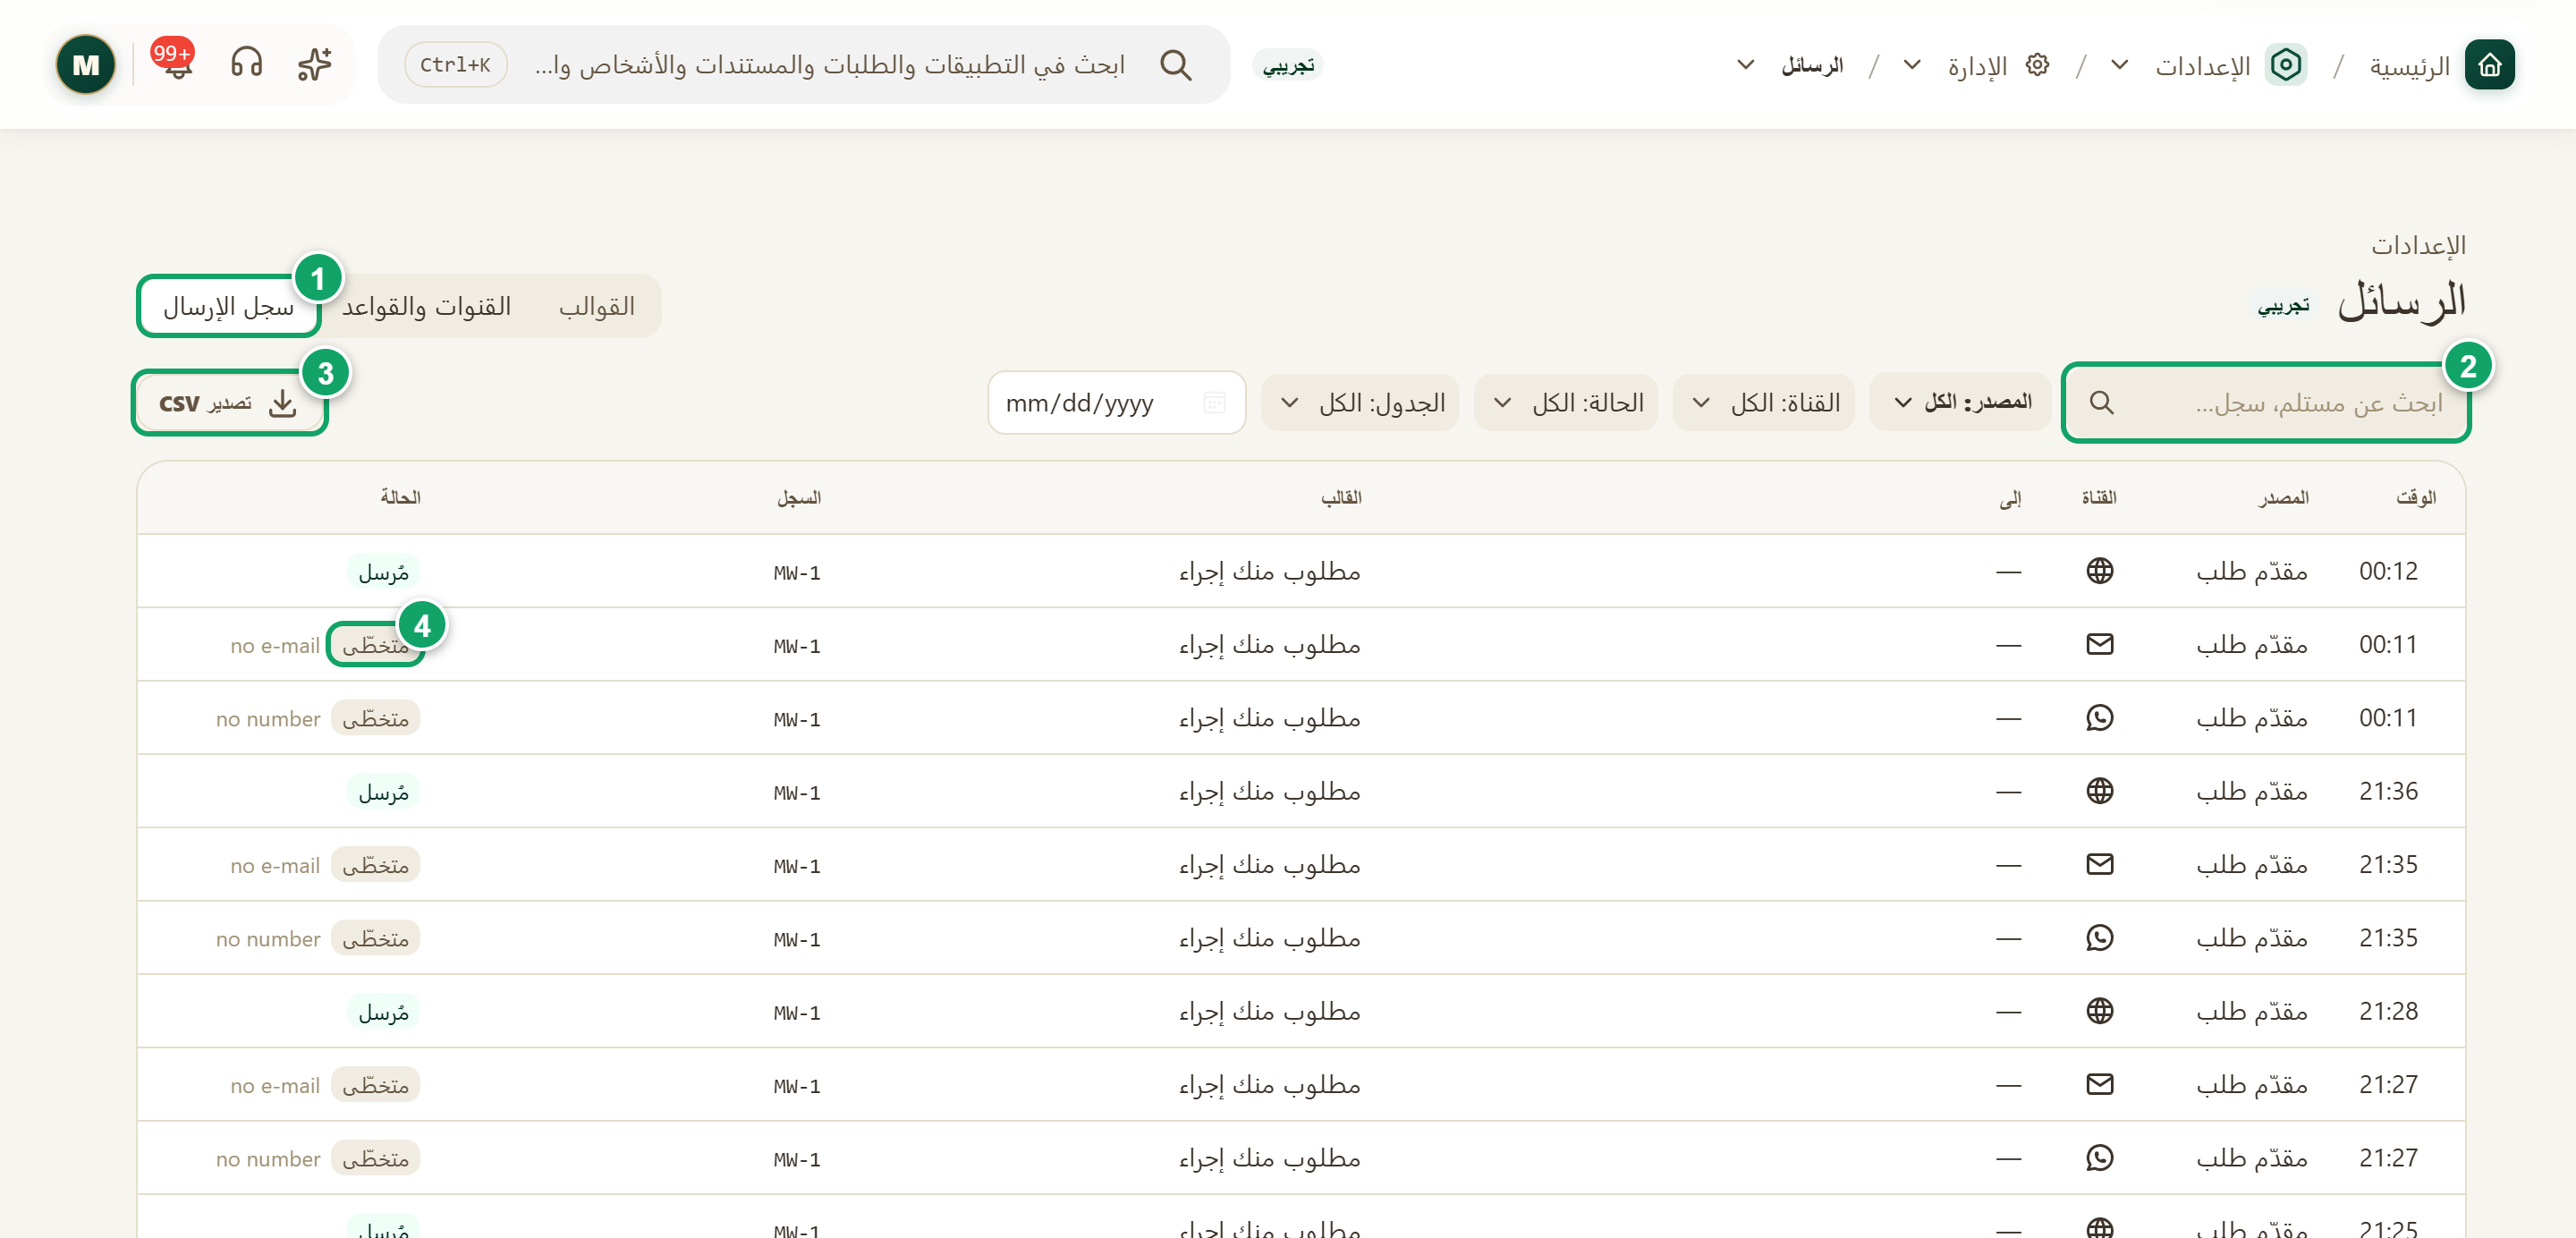
\includegraphics[width=0.95\linewidth,height=0.72\textheight,keepaspectratio]{figures/screens/ch08-messages-log-ar.png}
\caption{سجل الإرسال}
\label{fig:settings-messages-log}
\shotnote{يسجل السجل كل محاولة إرسال وقناتها وحالتها، فتعرف هل وصلت الرسالة إلى مرحلة الإرسال ولماذا تعذر ذلك. الصفوف الظاهرة بيانات اختبار. ① «سجل الإرسال». ② حقل البحث عن مستلم أو سجل. ③ «تصدير \en{CSV}»: يحفظ النتائج في ملف. ④ «متخطّى»: لم تُرسل الرسالة، ويظهر السبب بجوار الحالة.}
\end{figure}

\begin{table}[H]
\centering
\caption{ماذا تسجل في الرسائل؟}
\label{tab:settings-messages-fields}
\begin{tabularx}{\linewidth}{R{4.2cm} Y}
\rcHeaderRow
\thh{القسم} & \thh{ما الذي تسجله؟}\\
«أحداث مقدّمي الطلبات» & لكل حدث وقناة: تشغيل الإرسال أو إيقافه، والنص بالعربية والإنجليزية، و«استعادة النص الافتراضي» بعد تعديله. ولتذكير الزيارة تحدد عدد الأيام قبلها والساعة.\\
ما لا يُعدَّل هنا & نص واتساب في الأحداث قالب معتمد يُعدَّل خارج هذه الصفحة. أما حدث «رمز التحقق» فيظهر للاطلاع فقط.\\
«قوالب المتابعة» & المفتاح والاسم ونوع السجل والطرف المقابل، ثم نص كل قناة ولغة. يُنشر القالب، ويمر نص واتساب بمراجعة \en{Meta} قبل استخدامه.\\
«القنوات» & «اسم العرض في البريد» و«الرد إلى» و«اسم مُرسِل \en{SMS}»، إضافة إلى «إرسال بريد تجريبي» الذي يرسل رسالة حقيقية إلى العنوان الذي تكتبه.\\
«القواعد» & «ساعات الهدوء»، و«البديل بالبريد» عند تعذر واتساب أو الرسالة النصية، و«أسماء الأشهر العربية»، و«الحد الافتراضي لسلالم المتابعة الجديدة»، و«تتبّع التسليم / القراءة»، و«الاحتفاظ بمحتوى الرسائل لمدة».\\
«سجل الإرسال» & للاطلاع: البحث، والتصفية بالمصدر والقناة والحالة والجدول والتاريخ، وفتح تفاصيل الصف، وإعادة المحاولة عند توافرها.\\
\end{tabularx}
\end{table}

\begin{enumerate}
\item افتح «الإعدادات»، ثم «الرسائل».
\item اختر حدثاً من القائمة، ثم اختر القناة.
\item شغّل مفتاح القناة أو أوقفه، وعدّل النص بكل لغة. لا تعدّل المتغيرات بين القوسين.
\item اقرأ «المعاينة»، ثم اضغط «حفظ التغييرات».
\item افتح «القنوات والقواعد» واضبط «الرد إلى» وساعات الهدوء، ثم اضغط «حفظ التغييرات».
\end{enumerate}

\textbf{تحقق:} بعد الحفظ تُظهر قائمة الأحداث القنوات المفعّلة للحدث. وعند وصول حدث حقيقي، افتح «سجل الإرسال» واقرأ الحالة: «مُرسل» أو «فشل» أو «متخطّى» أو «مؤجّل»، واستخدم سبب التخطي لتعرف ما ينقص.
